
\documentclass{beamer}

\usetheme{default}
\usepackage{tikz}
\usetikzlibrary{arrows,shapes.arrows,positioning,shapes}
\usepackage{graphicx}
\usepackage{hyperref}
\newcommand\red[1]{{\color{red}#1}}
\newcommand\bred[1]{{\color{red}\textbf{#1}}}
\newcommand\blue[1]{{\color{blue}#1}}
\newcommand\bblue[1]{{\color{blue}\textbf{#1}}}
\newcommand\green[1]{{\color{olive}#1}}
\newcommand\bgreen[1]{{\color{olive}\textbf{#1}}}
\newcommand\black[1]{{\color{black}#1}}
\newcommand\white[1]{{\color{white}#1}}
\newcommand\E{\text{E}}
\newcommand\V{\text{V}}
\renewcommand\P{\text{P}}
\definecolor{seagreen4}{RGB}{46, 139, 87}


\setbeamertemplate{navigation symbols}{}
\setbeamertemplate{footline}[text line]{%
\parbox{\linewidth}{\vspace*{-8pt}Ian Lundberg (Princeton)}}

\newcommand{\indep}{{\bot\negthickspace\negthickspace\bot}}

\title{The Fragile Families Challenge:\\ \normalsize Predictability of family and child well-being in adolescence \vspace{-.2in}}

\author{\small Matthew J. Salganik, Ian Lundberg, Alex Kindel, Sara S. McLanahan,\\\small and 108 participants in the Fragile Families Challenge \vspace{-.05in}}

%\pgfdeclareimage[height=1cm]{university-logo}{ff_logo.jpg}
%\logo{\pgfuseimage{university-logo}}

%%%%%%%%%%%%%%%%%%%%%%%%%%%%%%
\begin{document}

%\begin{frame}
%  \titlepage
%\end{frame}

\begin{frame}
\centering
\begin{tikzpicture}[x = .5\textwidth, y = .5\textheight]
\node<1>[anchor = north] at (0,.9) {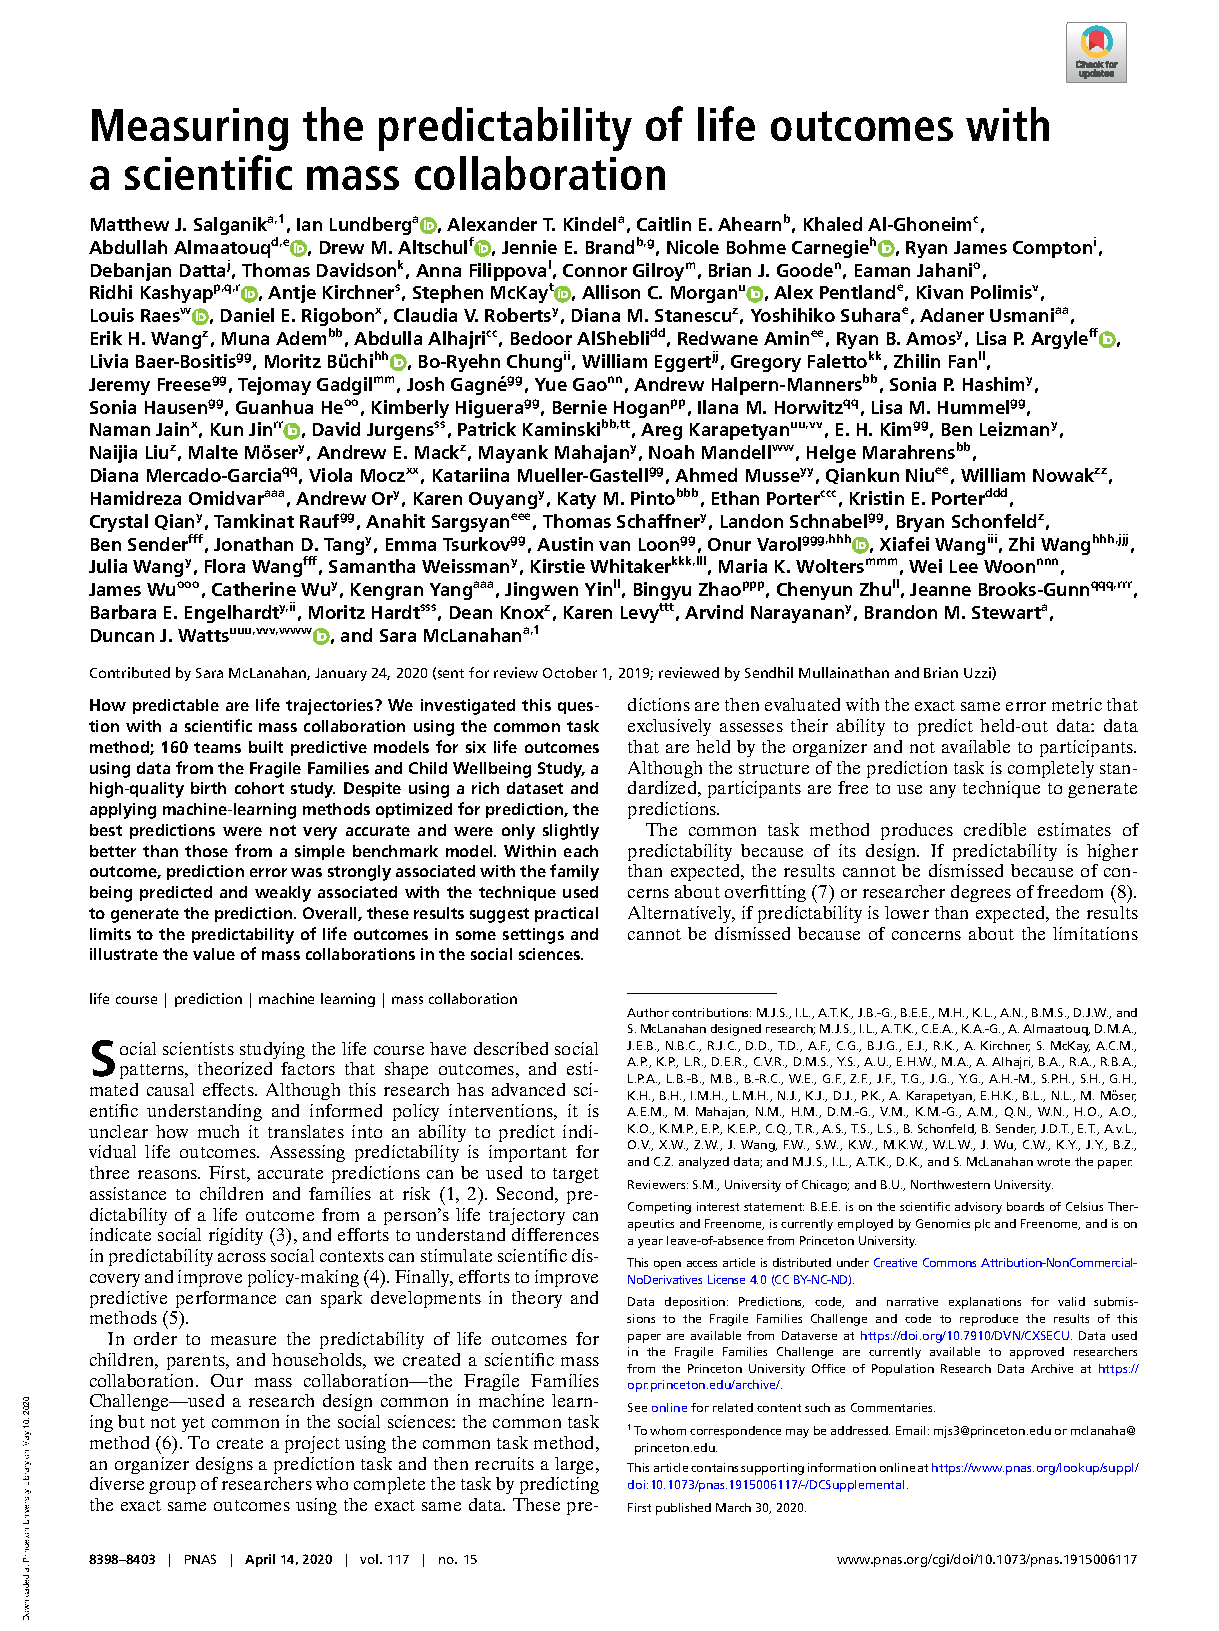
\includegraphics[width = \textwidth, trim = {0 9.5in 0 .6in}, clip]{figures/pnas_page1}};
\node<1>[align = center] at (0, .2) {Ian Lundberg\\Princeton University\\\\Berkeley Good Data Seminar\\12 May 2020};
\node<2->[anchor = north] at (0,.9) {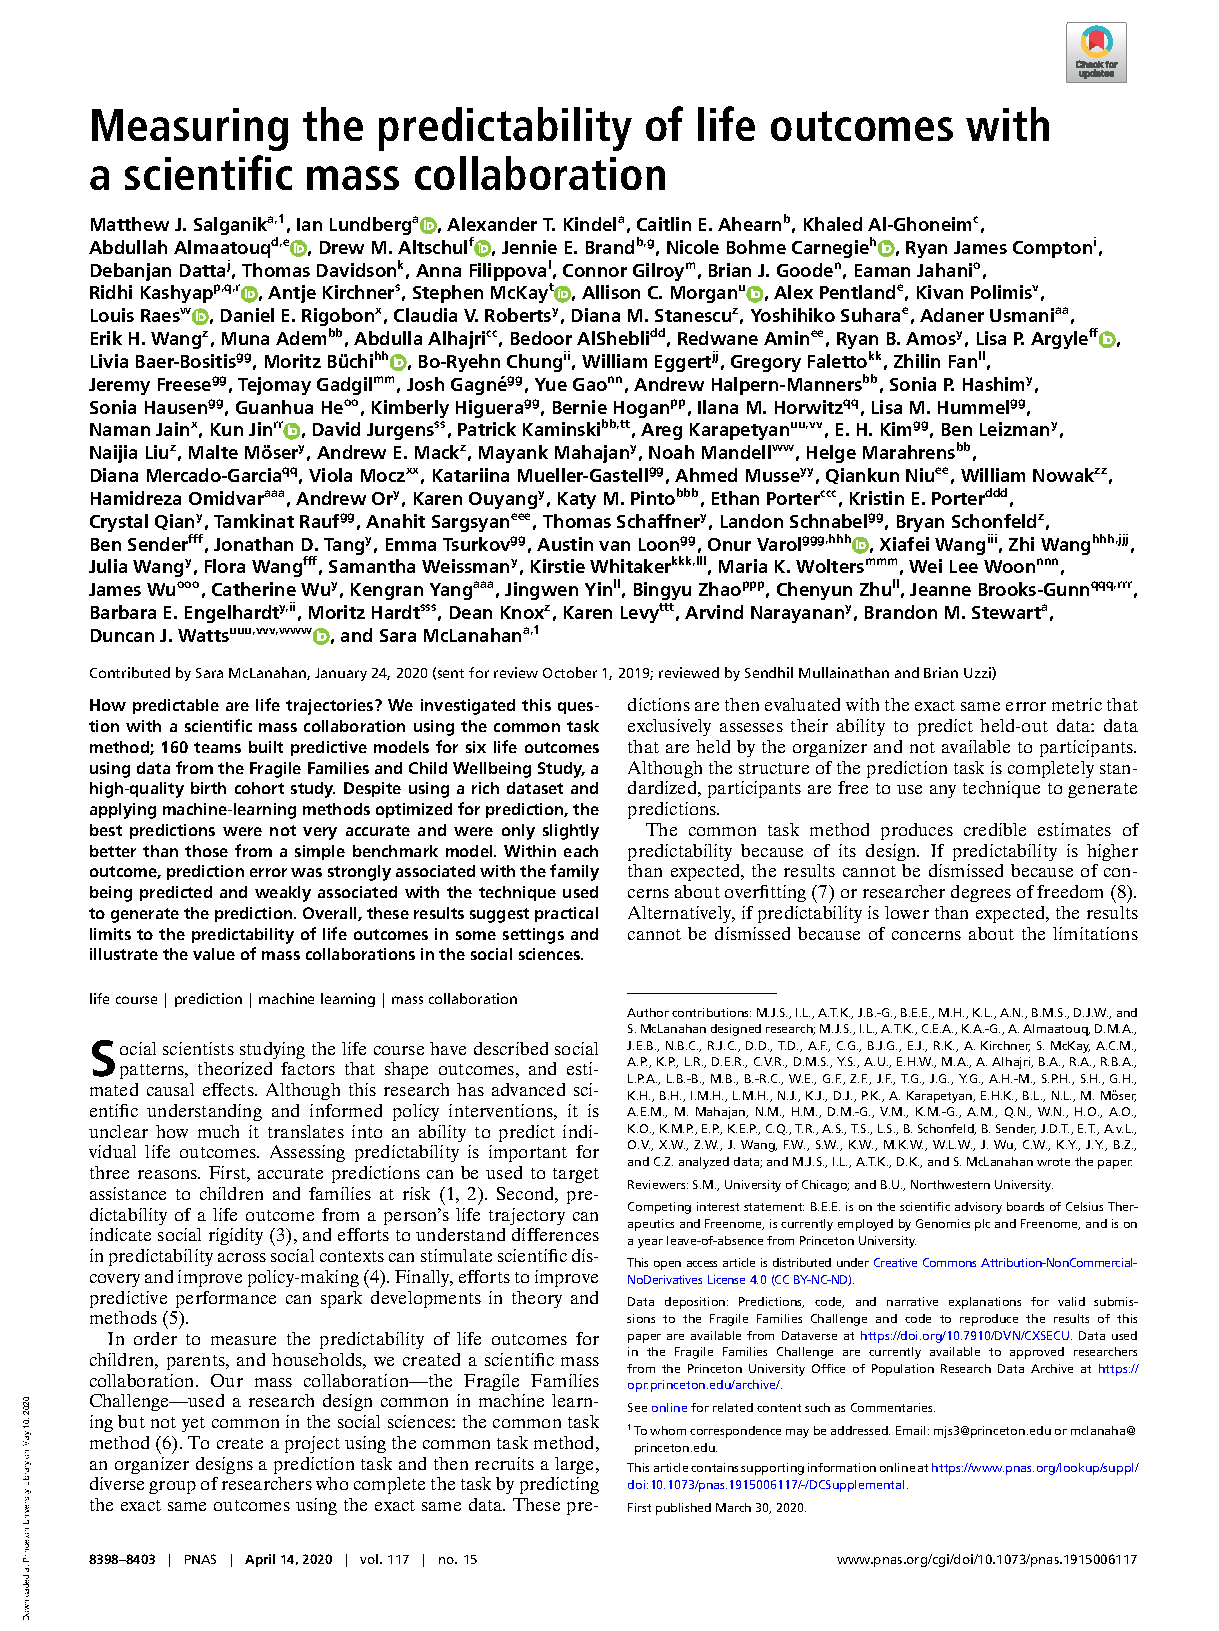
\includegraphics[width = \textwidth, trim = {0 6.5in 0 .6in}, clip]{figures/pnas_page1}};
%\node[align=center, font = \large, blue] at (0,.85) {Measuring the predictability of life outcomes\\with a scientific mass collaboration};
%\node[align = left, font = \footnotesize, anchor = north west] at (-1, .7) {Matthew J. Salganik, Ian Lundberg,\\Alex Kindel, Sara S. McLanahan,\\and 108 collaborators};
%\node[anchor = north east] at (1,.7) {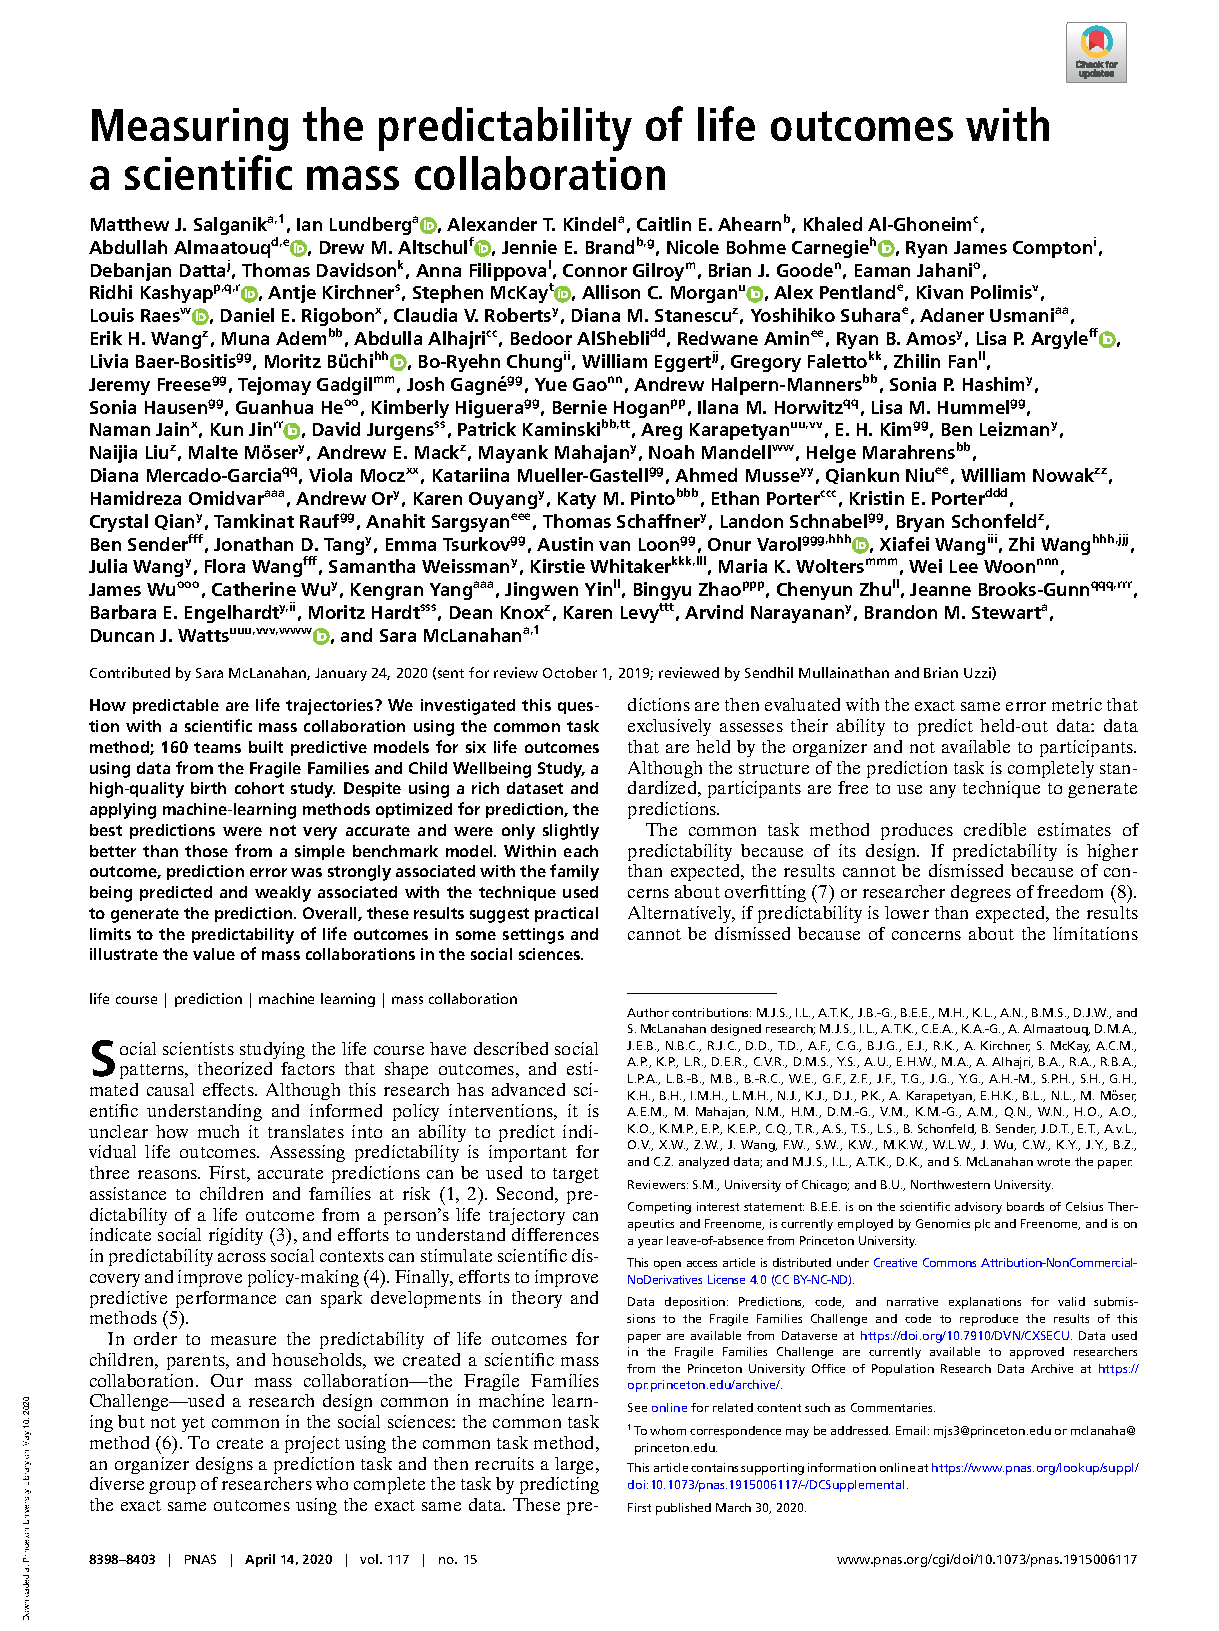
\includegraphics[width = .5\textwidth, trim = {0 6.5in 0 .6in}, clip]{figures/pnas_page1}};
%\node[align = left, anchor = west, font = \footnotesize] at (-1, .25) {Princeton University\\(+ many others)};
%\node[align = left, anchor = west, font = \footnotesize] at (-1, 0) {12 May 2020\\Berkeley Good Data Seminar};
\onslide<3>{
	%\draw[->, line width = 3pt, olive] (.9, 0) -- (.8, -.2);
	\draw[line width = 2pt, olive, rounded corners] (-1.05,-.77) rectangle (1.05,-.22);
}
\node[align = center, font = \scriptsize] at (0, -.5) {\begin{minipage}{\textwidth}This research is supported by the Russell Sage Foundation.  We are grateful to the members of the Board of Advisors of the Fragile Families Challenge: Jeanne Brooks-Gunn, Kathryn J. Edin, Barbara E. Engelhardt, Irwin Garfinkel, Moritz Hardt, Dean Knox, Nicholas Lemann, Karen Levy, Sara McLanahan, Arvind Narayanan, Timothy J. Nelson, Matthew Salganik, Brandon Stewart, \& Duncan Watts.\\Replication materials are on Dataverse: \textcolor{blue}{\textcolor{blue}{\href{https://doi.org/10.7910/DVN/CXSECU}{https://doi.org/10.7910/DVN/CXSECU}}}.\\Source for these slides: \textcolor{blue}{\textcolor{blue}{\href{http://github.com/fragilefamilieschallenge}{www.github.com/fragilefamilieschallenge}}}. 
\includegraphics[width=0.05\textwidth]{figures/cc.png}\end{minipage}};
\end{tikzpicture}
\end{frame}

\begin{frame}

\centering
\begin{tikzpicture}[x = \textwidth, y = \textheight]
\node at (0,0) {};
\node at (1,1) {};
% Life course visualization
\draw[->, line width = 2pt, gray] (.2,.85) -- (.8,.85);
\node[anchor = south] at (.5,.85) {Life course};
\node[anchor = north west, font = \footnotesize, align  = left] at (.2,.85) {Early\\experiences};
\node[anchor = north east, font = \footnotesize, align  = right] at (.8,.85) {Later\\outcomes};
% Standard approaches
\node<2->[anchor = north west, align = left] at (0,.7) {Standard social science practice};
\node<2->[anchor = west, font = \small] at (0,.6) {-- Describe social patterns};
\node<2->[anchor = west, font = \small] at (0,.55) {-- Theorize important factors};
\node<2->[anchor = west, font = \small] at (0,.5) {-- Estimate causal effects};
% Open questions
\node<3->[anchor = north west, align = left] at (.65,.7) {Open questions};
\node<4->[anchor = west, font = \small] at (.65,.6) {--};
\node<4->[anchor = west, font = \small, align = left] at (.68,.56) {Can we predict\\individual life\\outcomes?};
\node<5->[anchor = west, font = \small] at (.65,.45) {--};
\node<5->[anchor = west, font = \small, align = left] at (.68,.45) {Credibility};
% Illustration in data format
\node<6->[anchor = south, font = {\footnotesize\bf}] at (.35, .35) {Predictor variables};
\node<6->[anchor = south, font = {\footnotesize\bf}, rotate = 90] at (.1, .225) {Cases};
\draw<6->[rounded corners] (.1, .1) rectangle (.6,.35);
\node<6->[anchor = south, font = {\footnotesize\bf}] at (.8, .35) {Outcomes};
\draw<6->[rounded corners] (.7, .1) rectangle (.9,.35);
\draw<6->[->, line width = 4pt, gray] (.62, .225) -- (.68,.225);
% Illustrate picking a few predictors
\draw<7>[line width = 2pt, seagreen4] (.2,.1) -- (.2,.35);
\draw<7>[line width = 2pt, seagreen4] (.85,.1) -- (.85,.35);
\draw<8>[line width = 2pt, seagreen4] (.15,.1) -- (.15,.35);
\draw<8>[line width = 2pt, seagreen4] (.25,.1) -- (.25,.35);
\draw<8>[line width = 2pt, seagreen4] (.5,.1) -- (.5,.35);
\draw<8>[line width = 2pt, seagreen4] (.75,.1) -- (.75,.35);
\draw<9>[line width = 2pt, seagreen4] (.5,.1) -- (.5,.35);
\draw<9>[line width = 2pt, seagreen4] (.2,.1) -- (.2,.35);
\draw<9>[line width = 2pt, seagreen4] (.82,.1) -- (.82,.35);
\end{tikzpicture}

\end{frame}

\begin{frame}

\begin{center}

\includegraphics[width=\textwidth]{figures/ff_logo}
\end{center}

\begin{itemize}
\item Birth cohort panel study
\item $\approx$ 5,000 children born in 20 U.S. cities
\item Followed from birth through age 15
\end{itemize}

\end{frame}
%%%%%%%%%%%%%%%%%%%%%%%%%

\begin{frame}

\begin{center}
\includegraphics<1>[height=0.8\textheight]{figures/ff_design_public_b9}
\includegraphics<2>[height=0.8\textheight]{figures/ff_design_public2}
\end{center}

\end{frame}
%%%%%%%%%%%%%%%%%%%%%%%%%
\begin{frame}

Six age 15 outcomes:
\begin{itemize}
\item GPA
\item Material Hardship
\item Grit
\item Evicted
\item Job training
\item Job loss
\end{itemize}

\end{frame}
%%%%%%%%%%%%%%%%%%%%%%%%%
\begin{frame}

\begin{center}
%\includegraphics<1>[width=\textwidth]{figures/ff_design_matrix_ml}
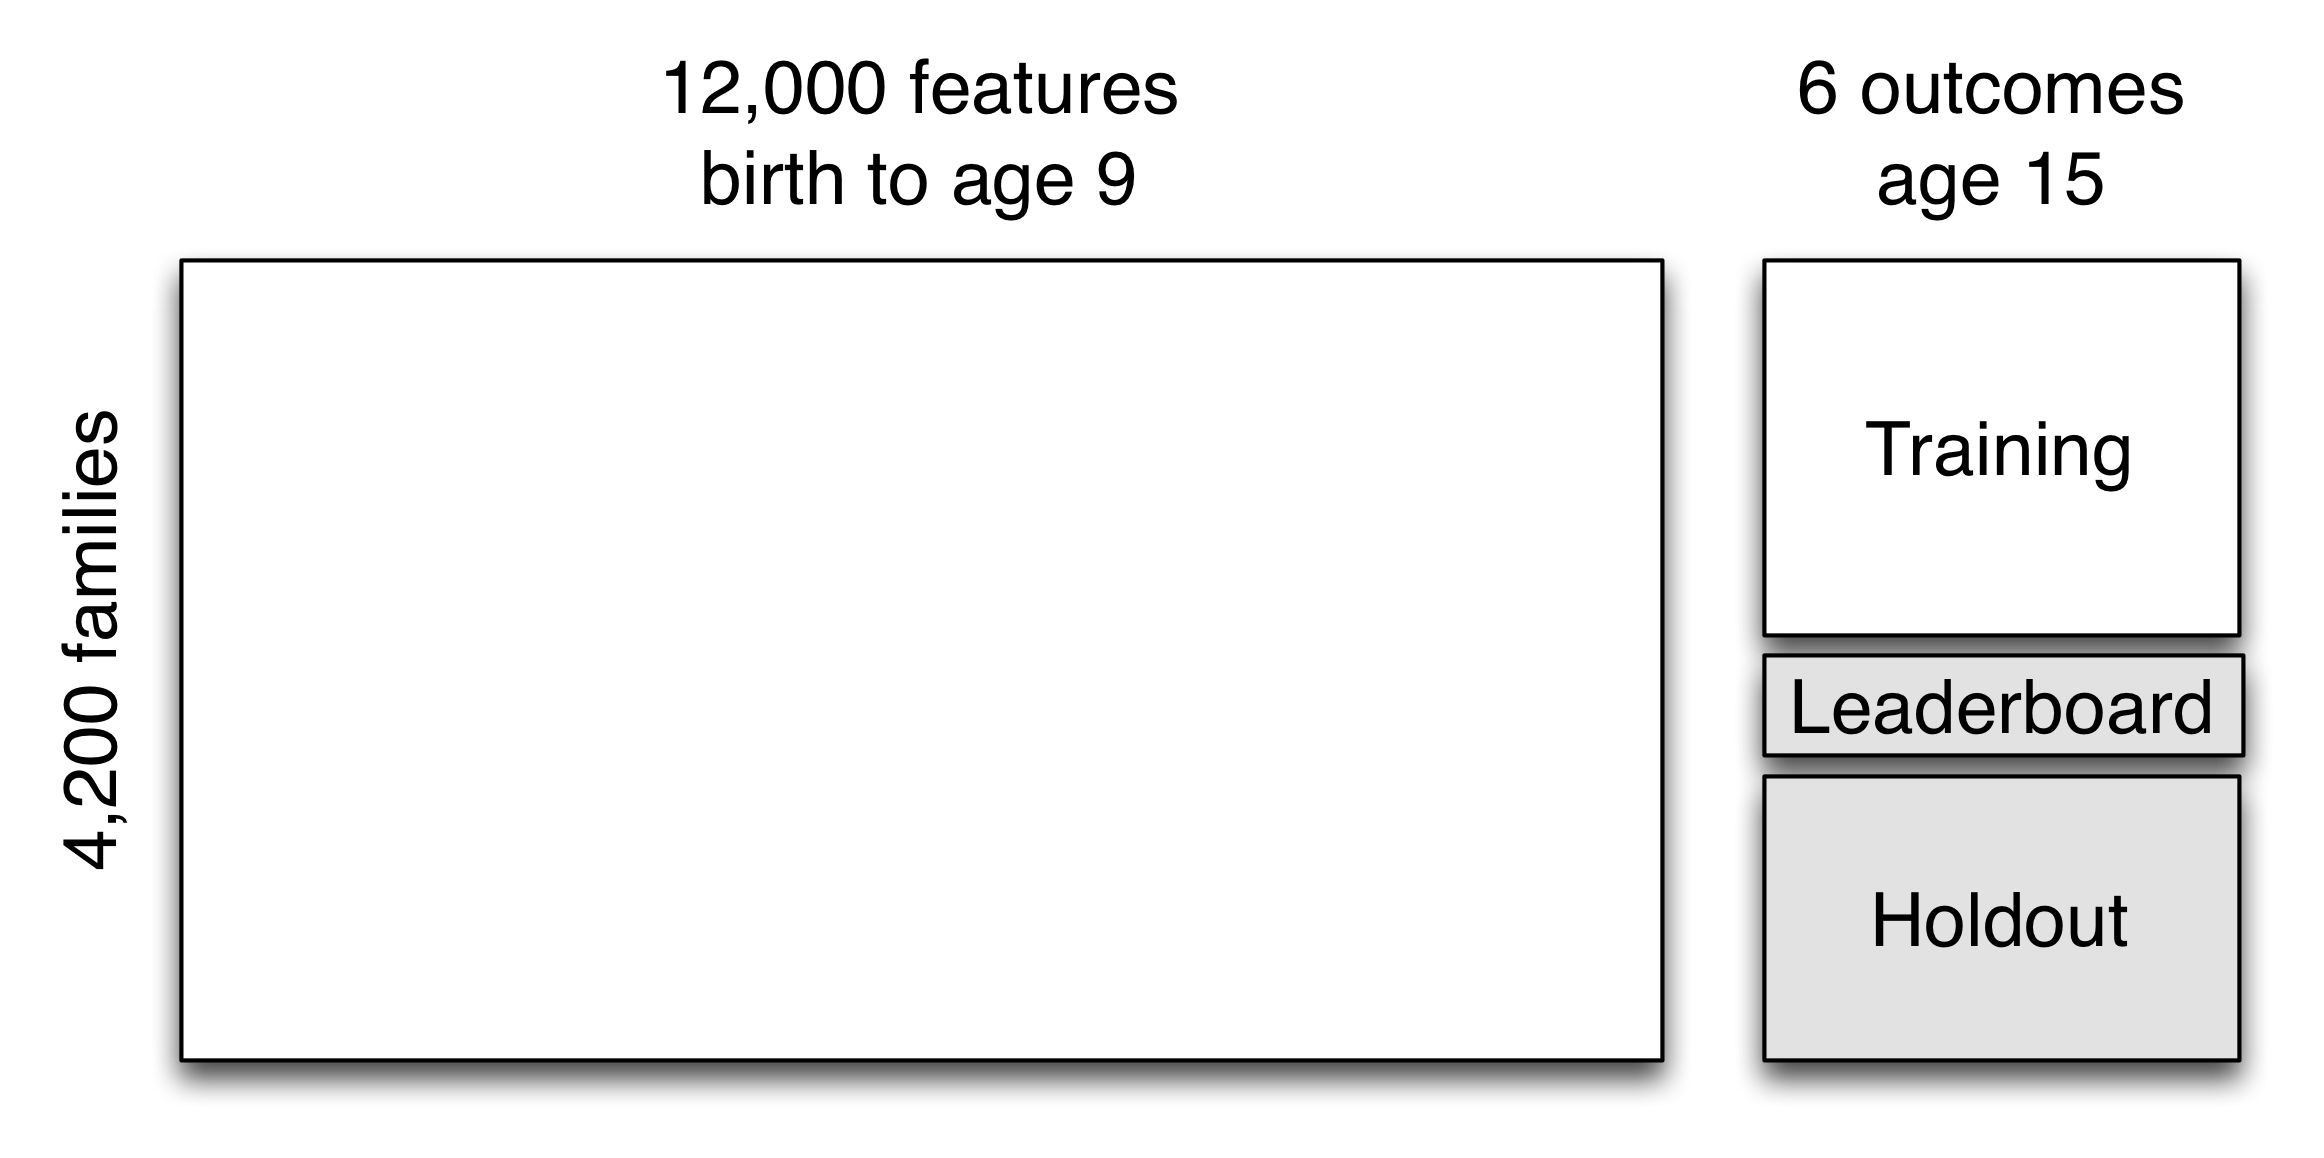
\includegraphics[width=\textwidth]{figures/ffc_design_matrix_ml}
\end{center}

\end{frame}
%%%%%%%%%%%%%%%%%%%%%%%%%
\begin{frame}

441 registered participants
\begin{itemize}
\item social scientists and data scientists
\item undergraduates, grad students, and professionals
\item many working in teams
\end{itemize}

\end{frame}
%%%%%%%%%%%%%%%%%%%%%%%%%%%
\begin{frame}

\begin{center}
How did they do?
\end{center}

\end{frame}
%%%%%%%%%%%%%%%%%%%%%%%%%%%
\begin{frame}
\centering
\begin{tikzpicture}[x = \textwidth, y = \textheight]
\node<1>[anchor = north] at (.5,1) {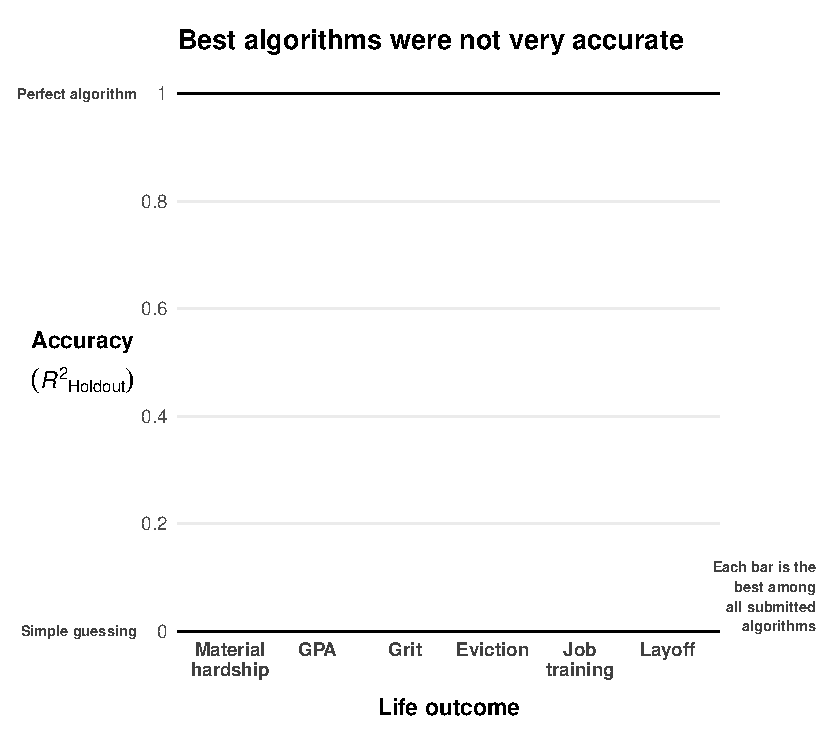
\includegraphics[width=\textwidth]{figures/image0}};
\draw<1>[fill = white, color = white] (.2,.9) rectangle (.85,.95);
\node<1> at (.55,.5) {$R^2_\text{Holdout} = 1 - \frac{\sum_{i\in\text{Holdout}} \left(y_i - \hat{y}_i\right)^2}{\sum_{i\in\text{Holdout}} \left(y_i - \bar{y}_\text{Training}\right)^2}$};
\node<2-6>[anchor = north] at (.5,1) {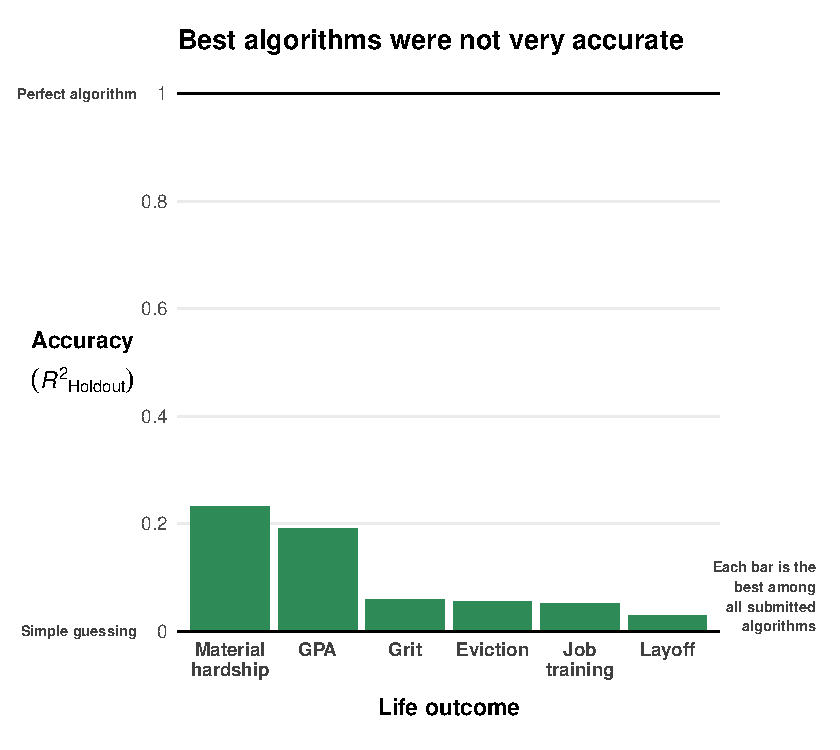
\includegraphics[width=\textwidth]{figures/image1}};
\node<3>[draw, rounded corners, fill = white] at (.63,.55) {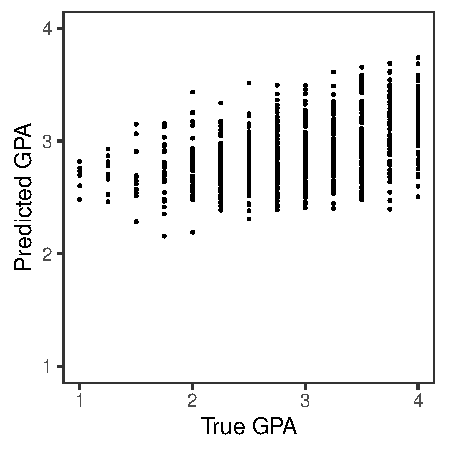
\includegraphics[height = .5\textheight]{figures/gpa_best_scatter}};
\node<4>[draw, rounded corners, fill = white] at (.63,.55) {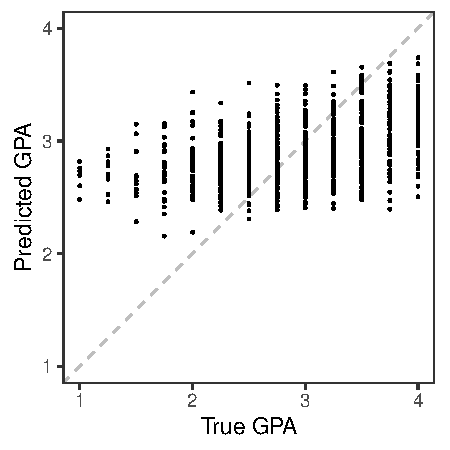
\includegraphics[height = .5\textheight]{figures/gpa_best_scatter_diagonal}};
\node<5>[draw, rounded corners, fill = white] at (.63,.55) {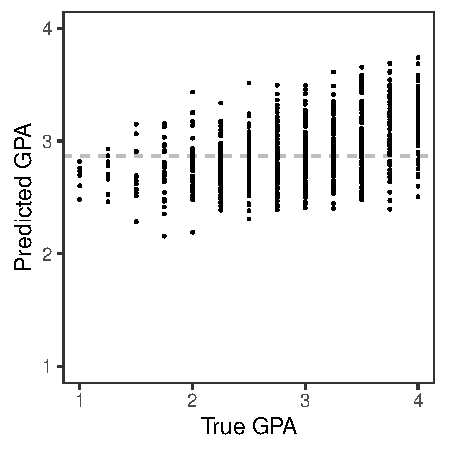
\includegraphics[height = .5\textheight]{figures/gpa_best_scatter_horizontal}};
\node<7>[anchor = north] at (.5,1) {\includegraphics[width=\textwidth]{figures/image1a}};
\end{tikzpicture}
\end{frame}

%%%%%%%%%%%%%%%%%%%%%%%%%%%
\begin{frame}
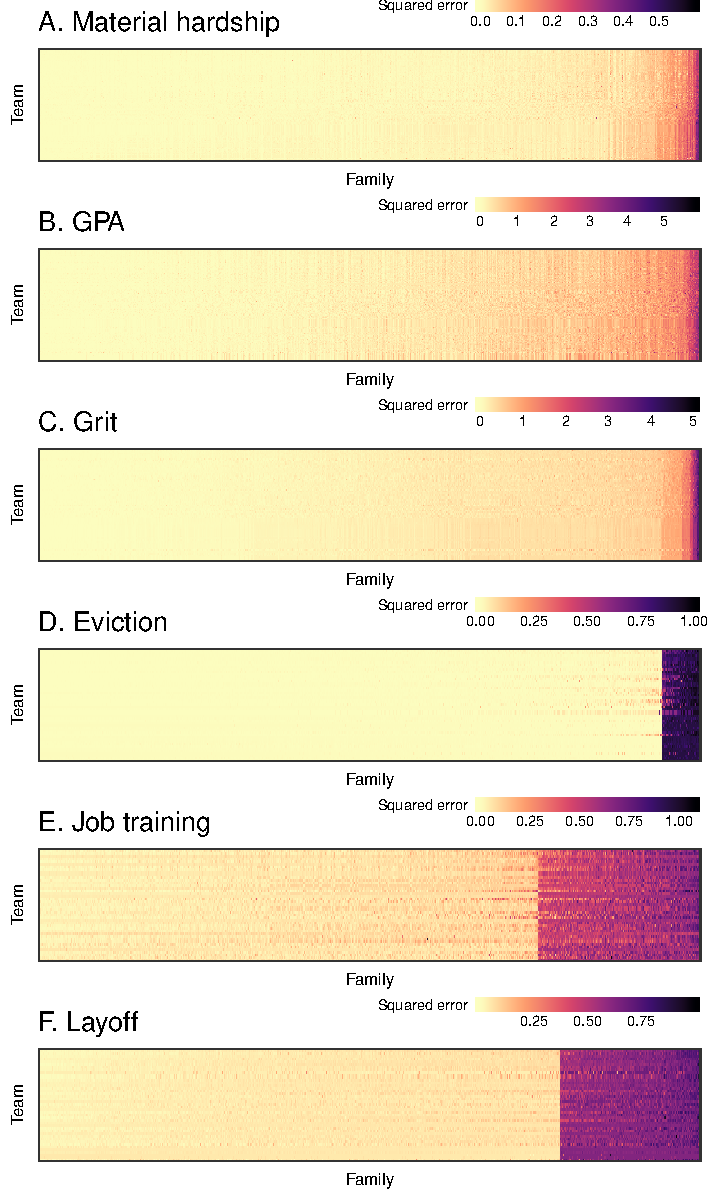
\includegraphics[width = \textwidth, trim = {0 5.37in 0 1.3in}, clip]{figures/4_heatmaps_sqerr_6outcomes}
\end{frame}

%%%%%%%%%%%%%%%%%%%%%%%%%%%
\begin{frame}
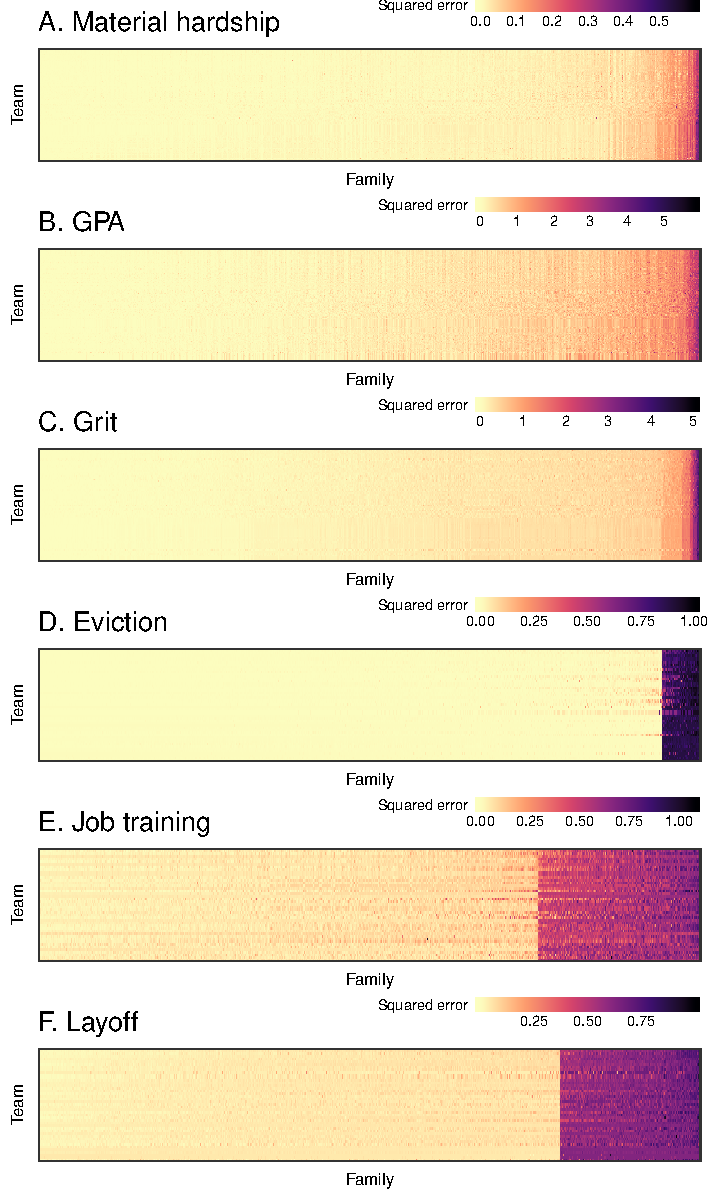
\includegraphics[width = \textwidth, trim = {0 2.72in 0 3.95in}, clip]{figures/4_heatmaps_sqerr_6outcomes}
\end{frame}

%%%%%%%%%%%%%%%%%%%%%%%%%%%
\begin{frame}
% Blank slide for separation
\end{frame}

%%%%%%%%%%%%%%%%%%%%%%%%%%%
\begin{frame}
What do these results mean for policy and for science?
\end{frame}

%%%%%%%%%%%%%%%%%%%%%%%%%%%
\begin{frame}
\begin{tikzpicture}[x = \textwidth, y = \textheight]
\node at (0,0) {};
\node at (1,1) {};
\node[anchor = north west, align = left] at (0,.83) {For \bblue{policymakers},};
\node<2->[anchor = north west, align = left] at (0,.68) {-- Do not assume that predictive algorithms are accurate};
\node<3->[anchor = north west, align = left] at (0,.58) {-- Transparent evaluation of any algorithm is needed};
\node<4->[anchor = north west, align = left] at (0,.48) {-- Complex models may not outperform simple models};
\end{tikzpicture}
\end{frame}

%%%%%%%%%%%%%%%%%%%%%%%%%%%
\begin{frame}
\begin{tikzpicture}[x = \textwidth, y = \textheight]
\node at (0,0) {};
\node at (1,1) {};
\node[anchor = north west] at (0,.95) {For \bblue{scientists}: A paradox of prediction and understanding};
\node<2->[anchor = north west, align = left] at (0,.83) {These data have\\generated\\understanding...};
\node<2->[anchor = north, font = \footnotesize] at (0.15,.63) {(hundreds of papers)};
\draw<2->[->, thick] (.15,.63) -- (.13,.66);
\node<3->[anchor = north east, align = right] at (1,.83) {...yet the very same data\\did not yield accurate\\predictions};
\node<3->[anchor = north, font = \footnotesize] at (0.85,.63) {(our result)};
\draw<3->[->, thick] (.85,.63) -- (.87,.66);
\node<4->[anchor = north west, align = left] at (0,.52) {\bblue{Resolutions:}};
\node<5->[anchor = north east, font = \small] at (0.04,.45) {1. };
\node<5->[anchor = north west, align = left, font = \small] at (.04,.45) {If understanding implies an ability to predict,\\then \bgreen{we do not understand} the life course.};
\node<6->[anchor = north east, font = \small] at (0.04,.34) {2. };
\node<6->[anchor = north west, align = left, font = \small] at (.04,.34) {Perhaps we have \bgreen{understanding despite poor prediction}.};
\node<6->[anchor = north west, align = left, font =  \footnotesize] at (.06,.29) {-- Aggregate description\\-- Causal effects};
\node<7->[anchor = north east, font = \small] at (0.04,.18) {3. };
\node<7->[anchor = north west, align = left, font = \small] at (.04,.18) {Our understanding is correct but \bgreen{incomplete}.\\We need theories that point toward poor prediction};
\end{tikzpicture}
\end{frame}

%%%%%%%%%%%%%%%%%%%%%%%%%%%
\begin{frame}
\begin{tikzpicture}[x = \textwidth, y = \textheight]
\node at (0,0) {};
\node at (1,1) {};
\node[anchor = north west] at (0,.95) {For \bblue{scientists}: The value of mass collaboration};
\node<2->[anchor = south west, align = left] at (0, .65) {A credible estimate of predictability};
\node<3->[anchor = west, align = left] at (0, .5) {The common task framework does not end\\with choosing the winner};
\node<4->[anchor = north west, align = left] at (0, .35) {There may be other problems we can solve\\better collectively than individually};
\end{tikzpicture}
\end{frame}

%%%%%%%%%%%%%%%%%%%%%%%%%%%
\begin{frame}
\centering
\includegraphics[width=\textwidth]{figures/image1a}

\end{frame}

%%%%%%%%%
%  APPENDIX	%
%%%%%%%%%

\begin{frame}
\centering \huge Appendix
\end{frame}

\begin{frame}{Appendix}
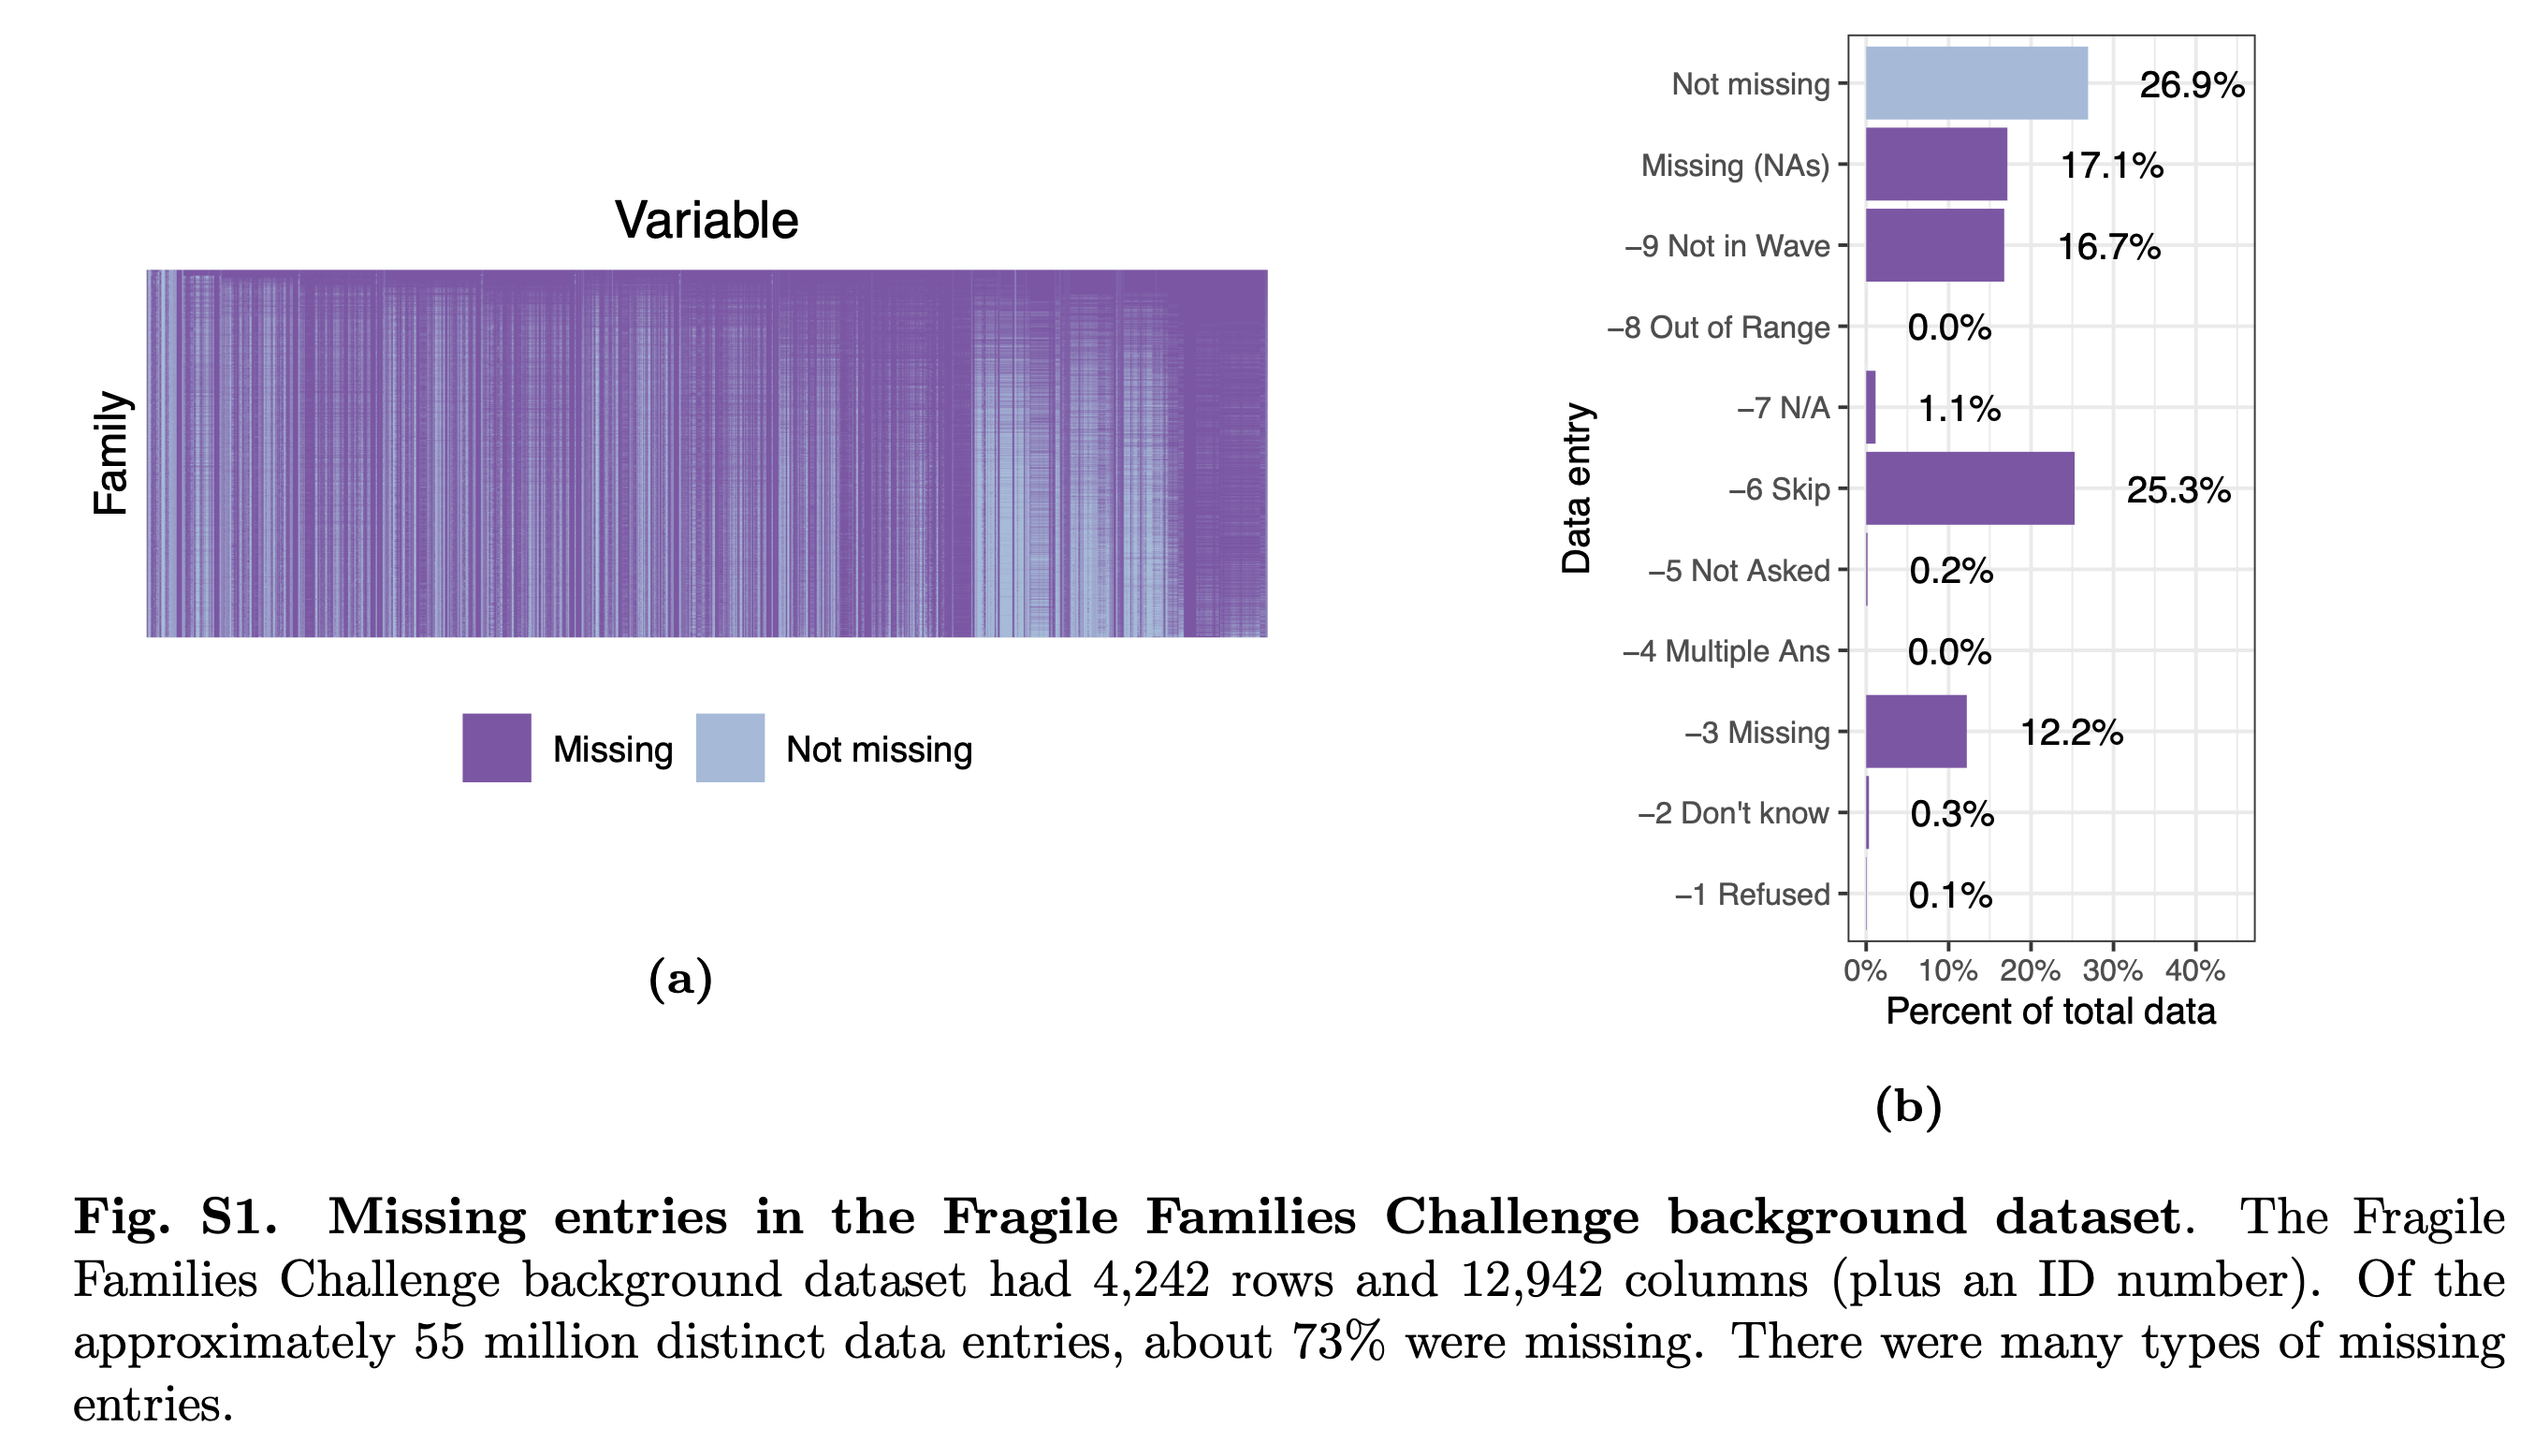
\includegraphics[width = \textwidth]{figures/si_missing_data}
\end{frame}

\begin{frame}{Appendix}
\centering
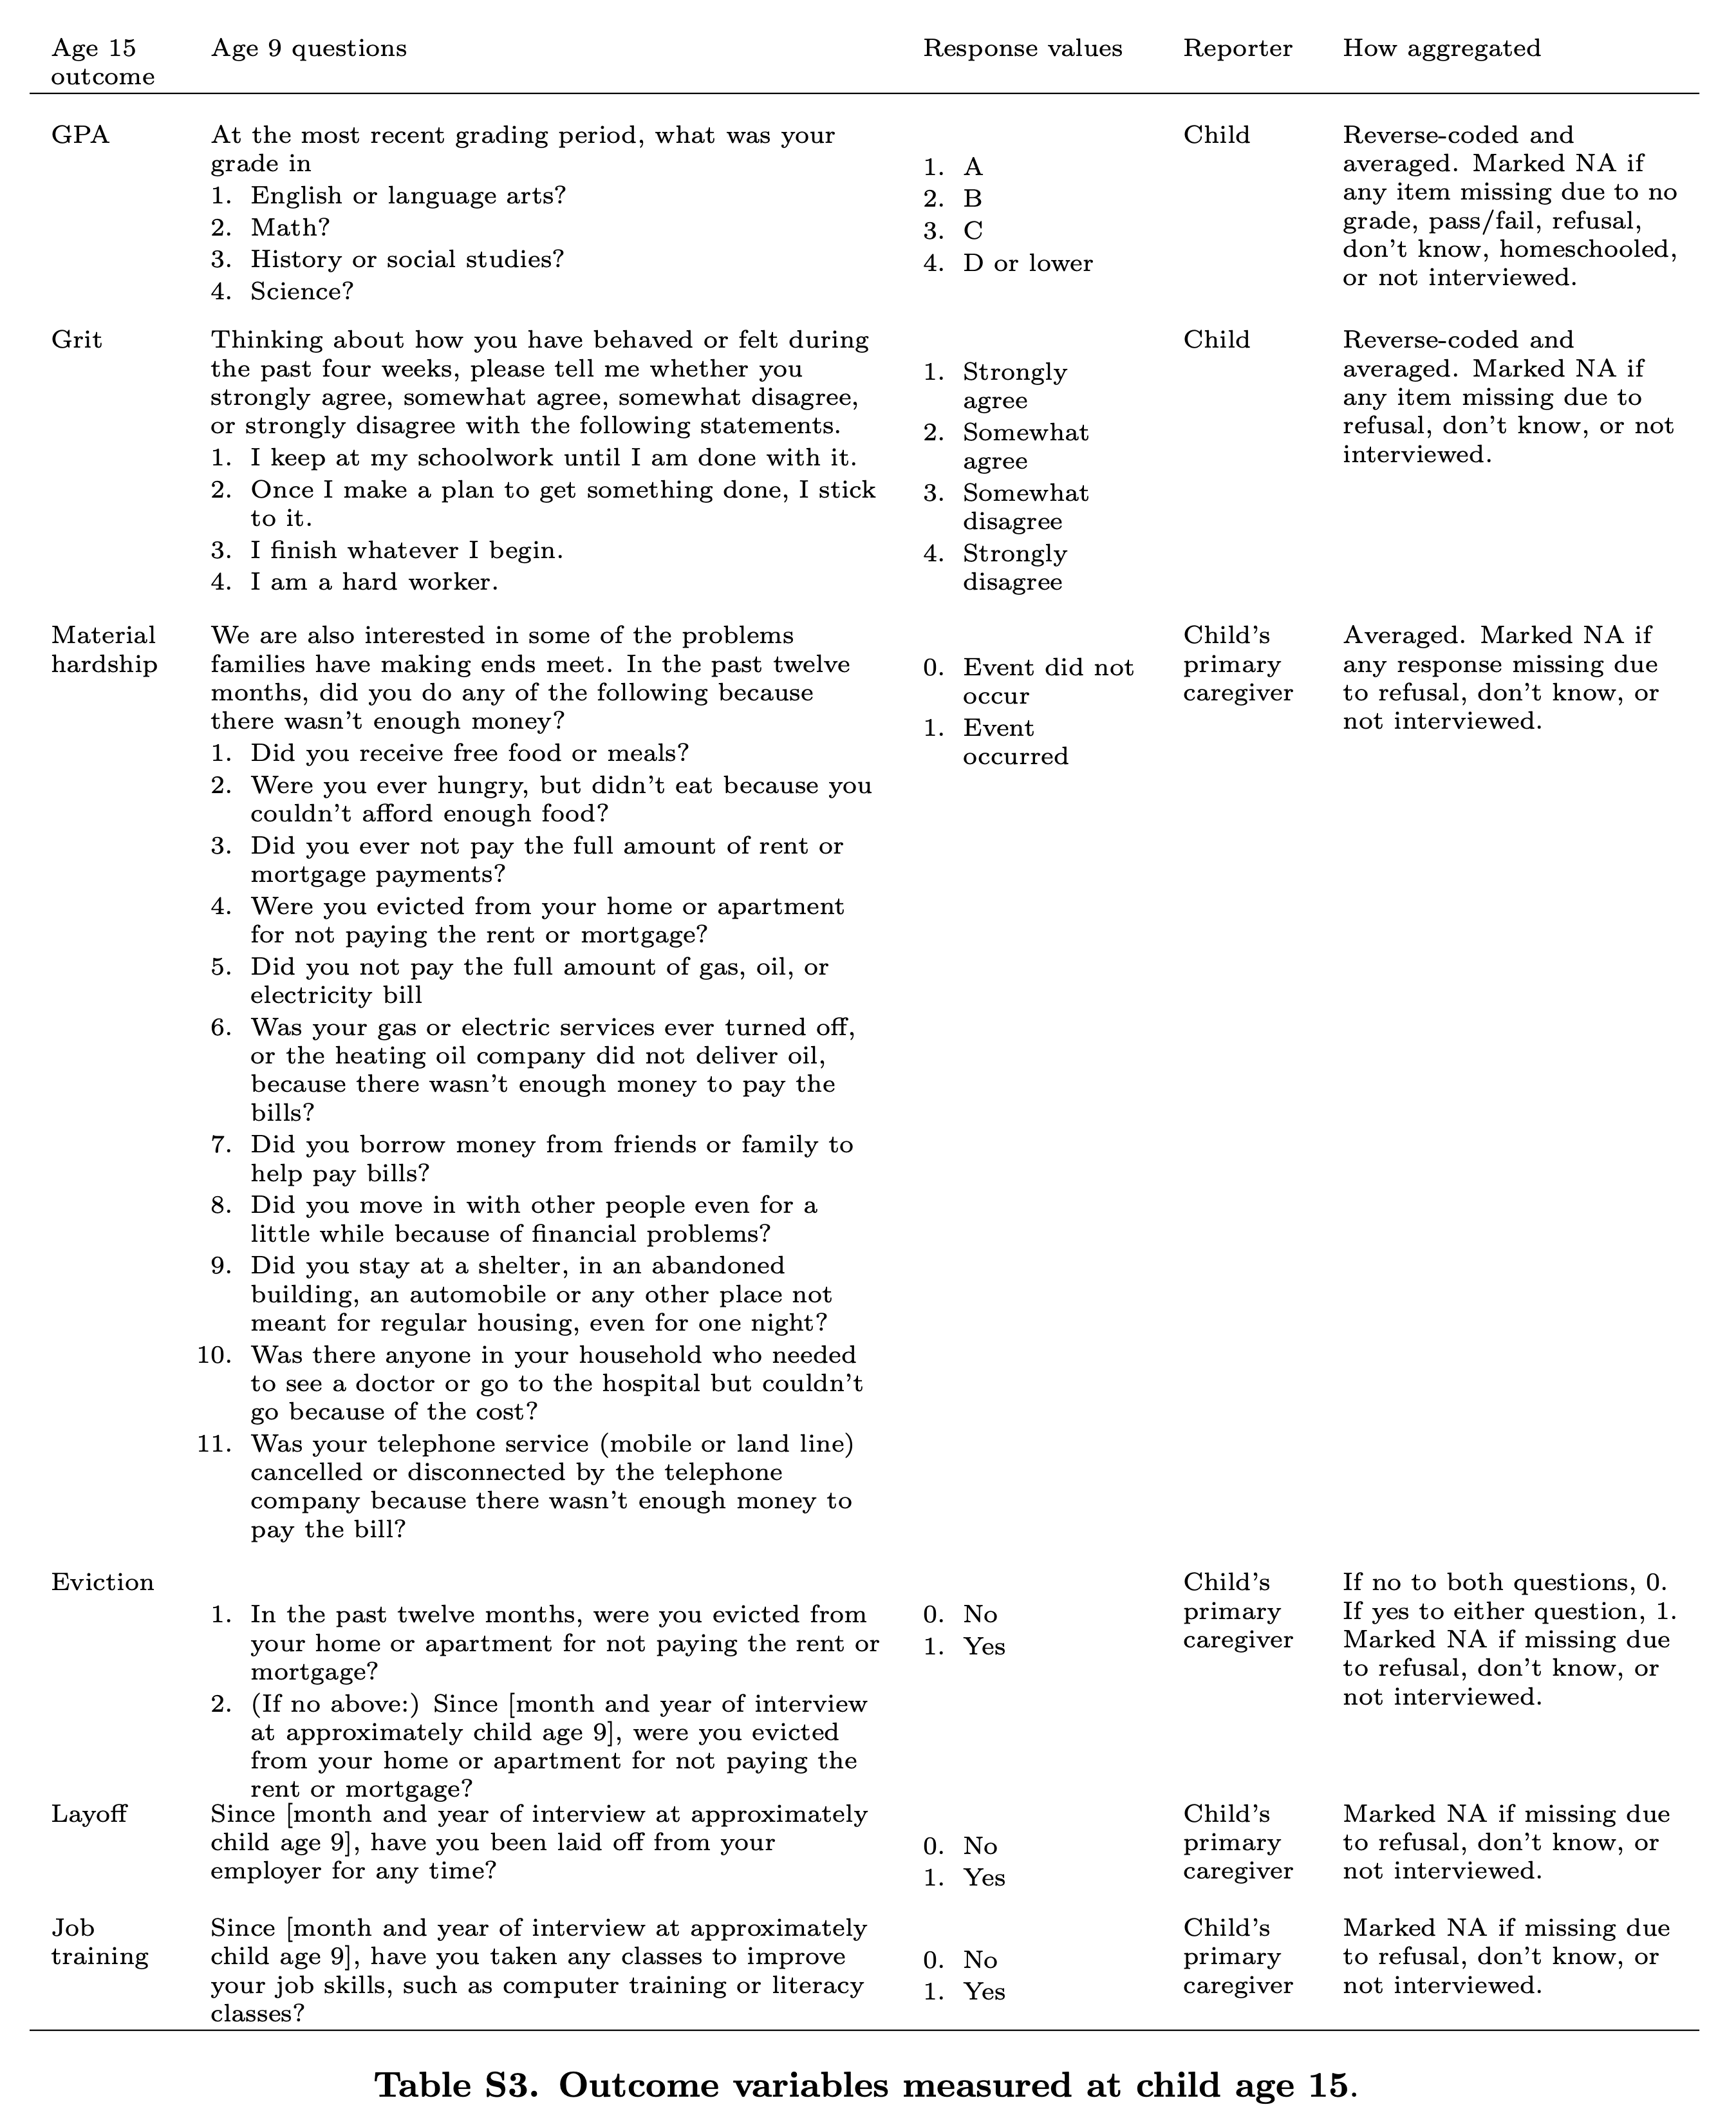
\includegraphics[height = .8\textheight]{figures/si_outcome_text}
\end{frame}

\begin{frame}{Appendix}
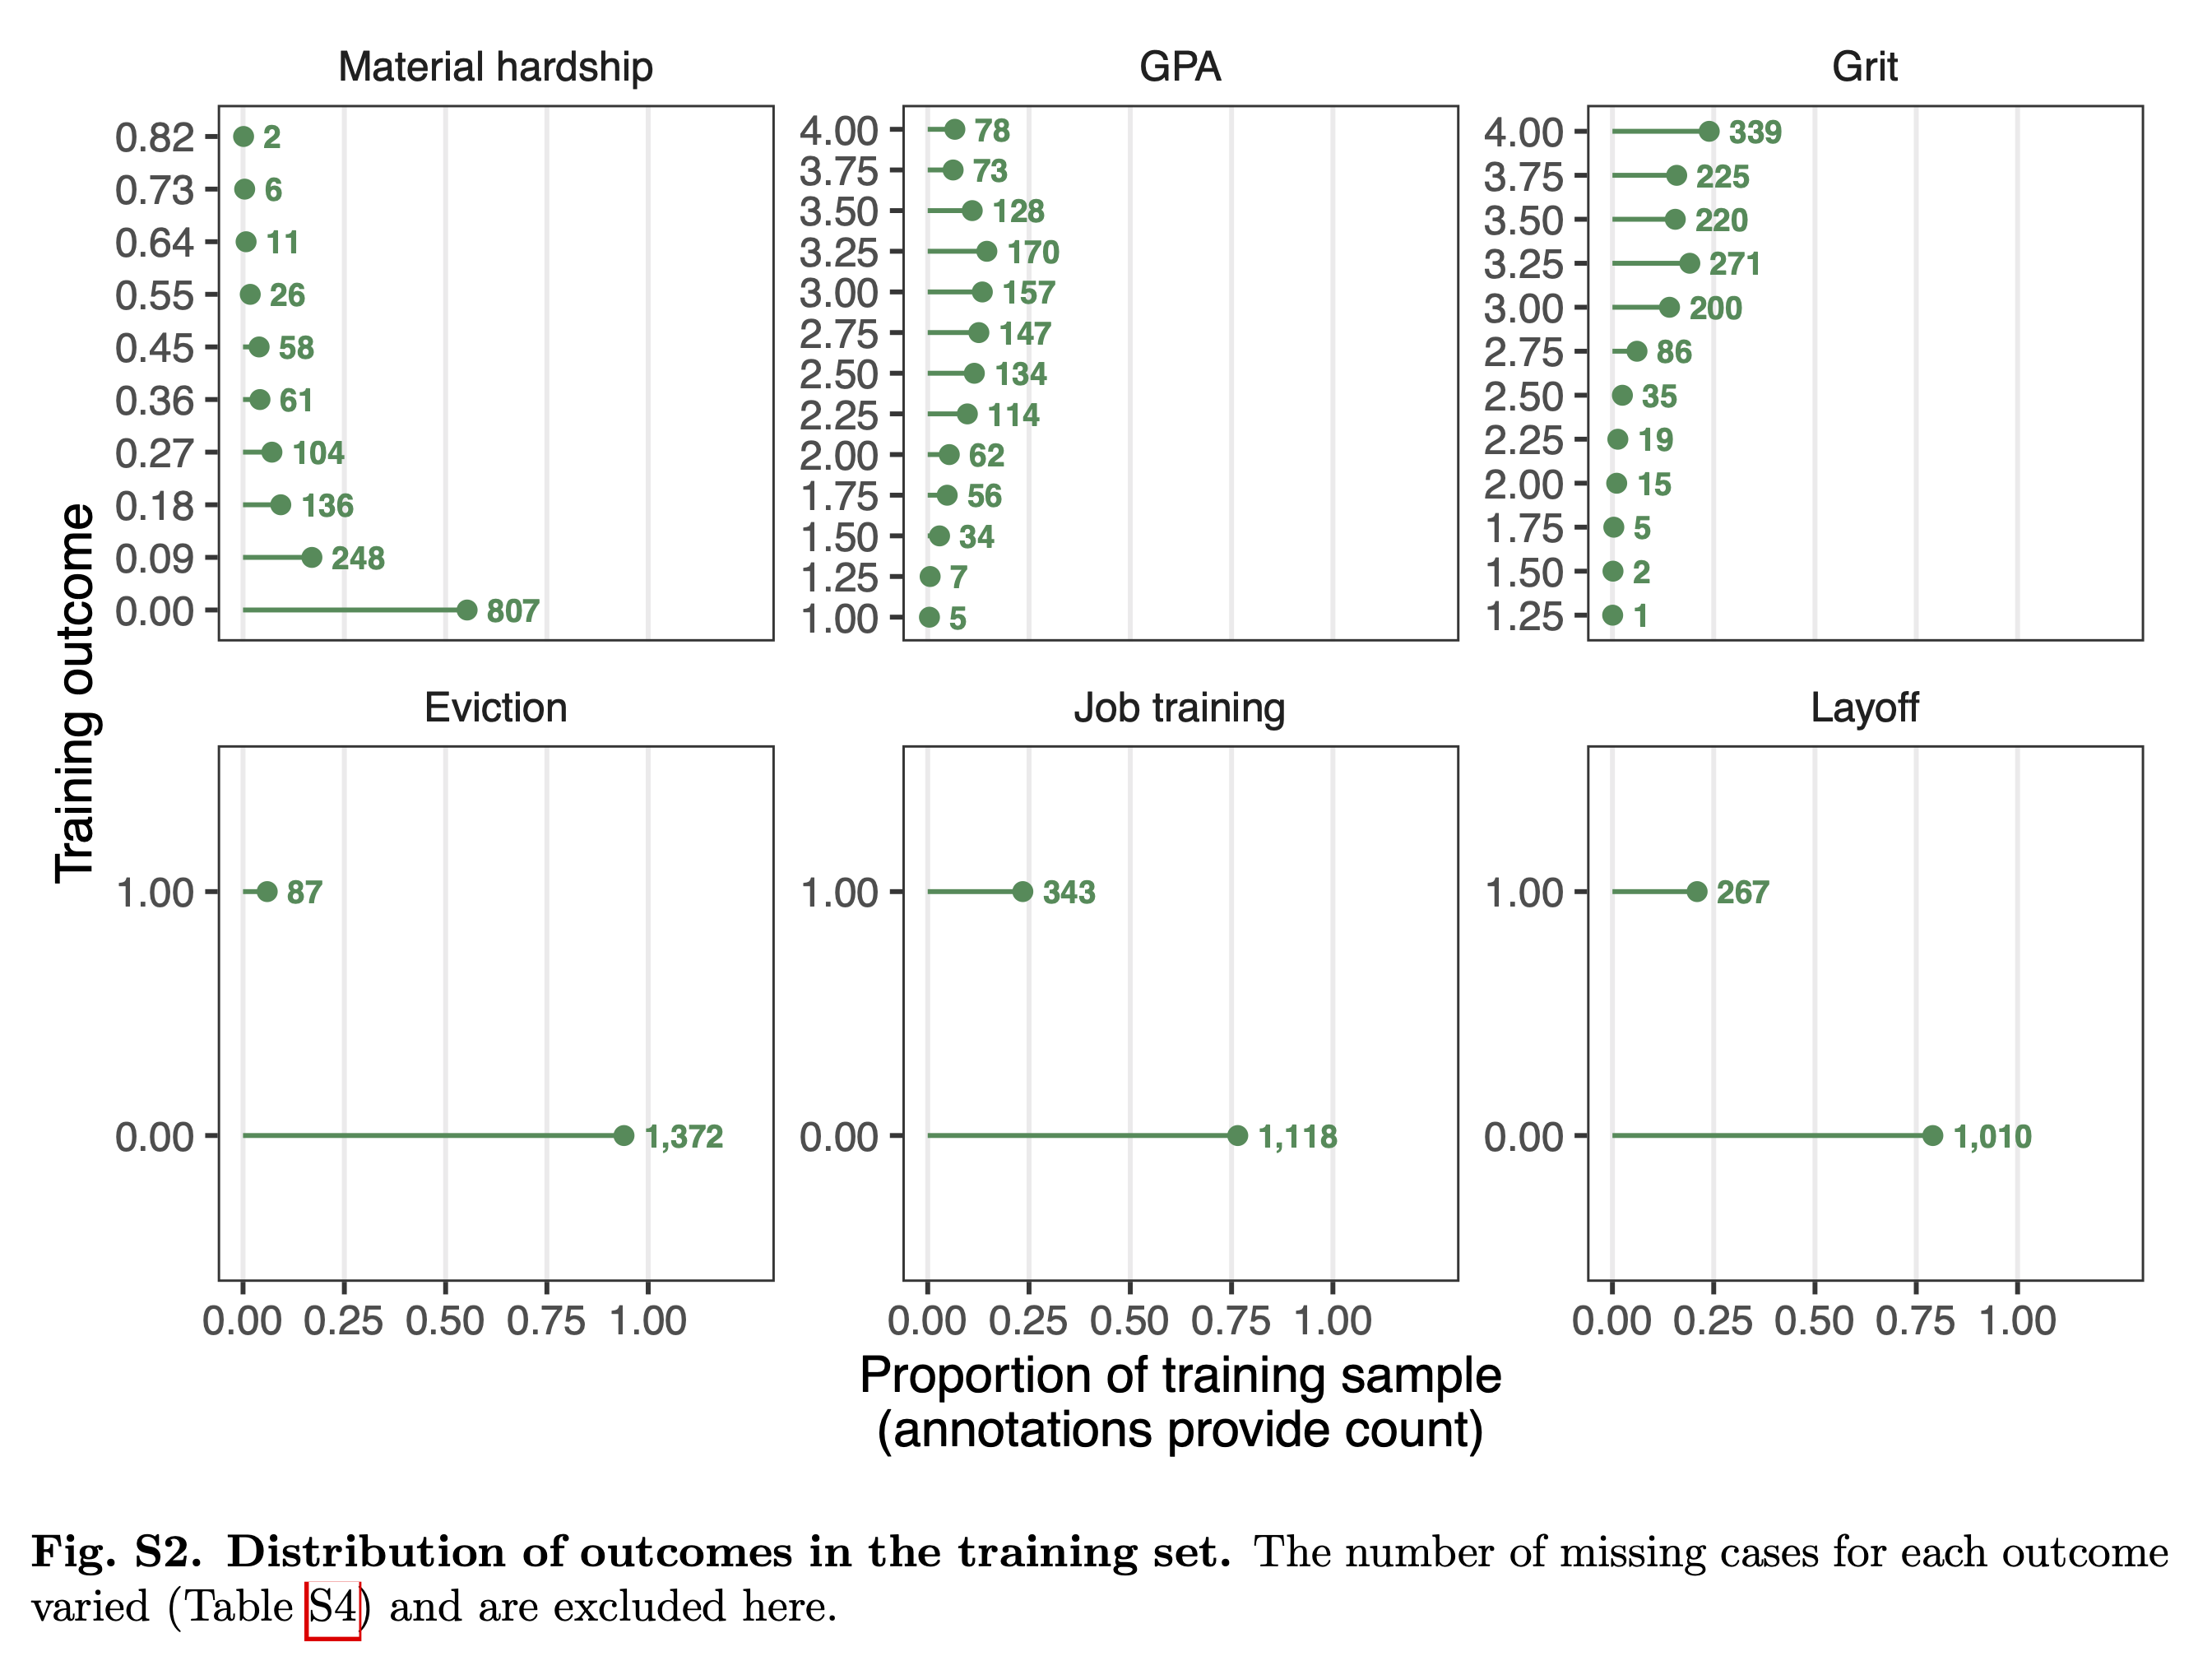
\includegraphics[width = \textwidth]{figures/si_outcome_histograms}
\end{frame}

\begin{frame}{Appendix}
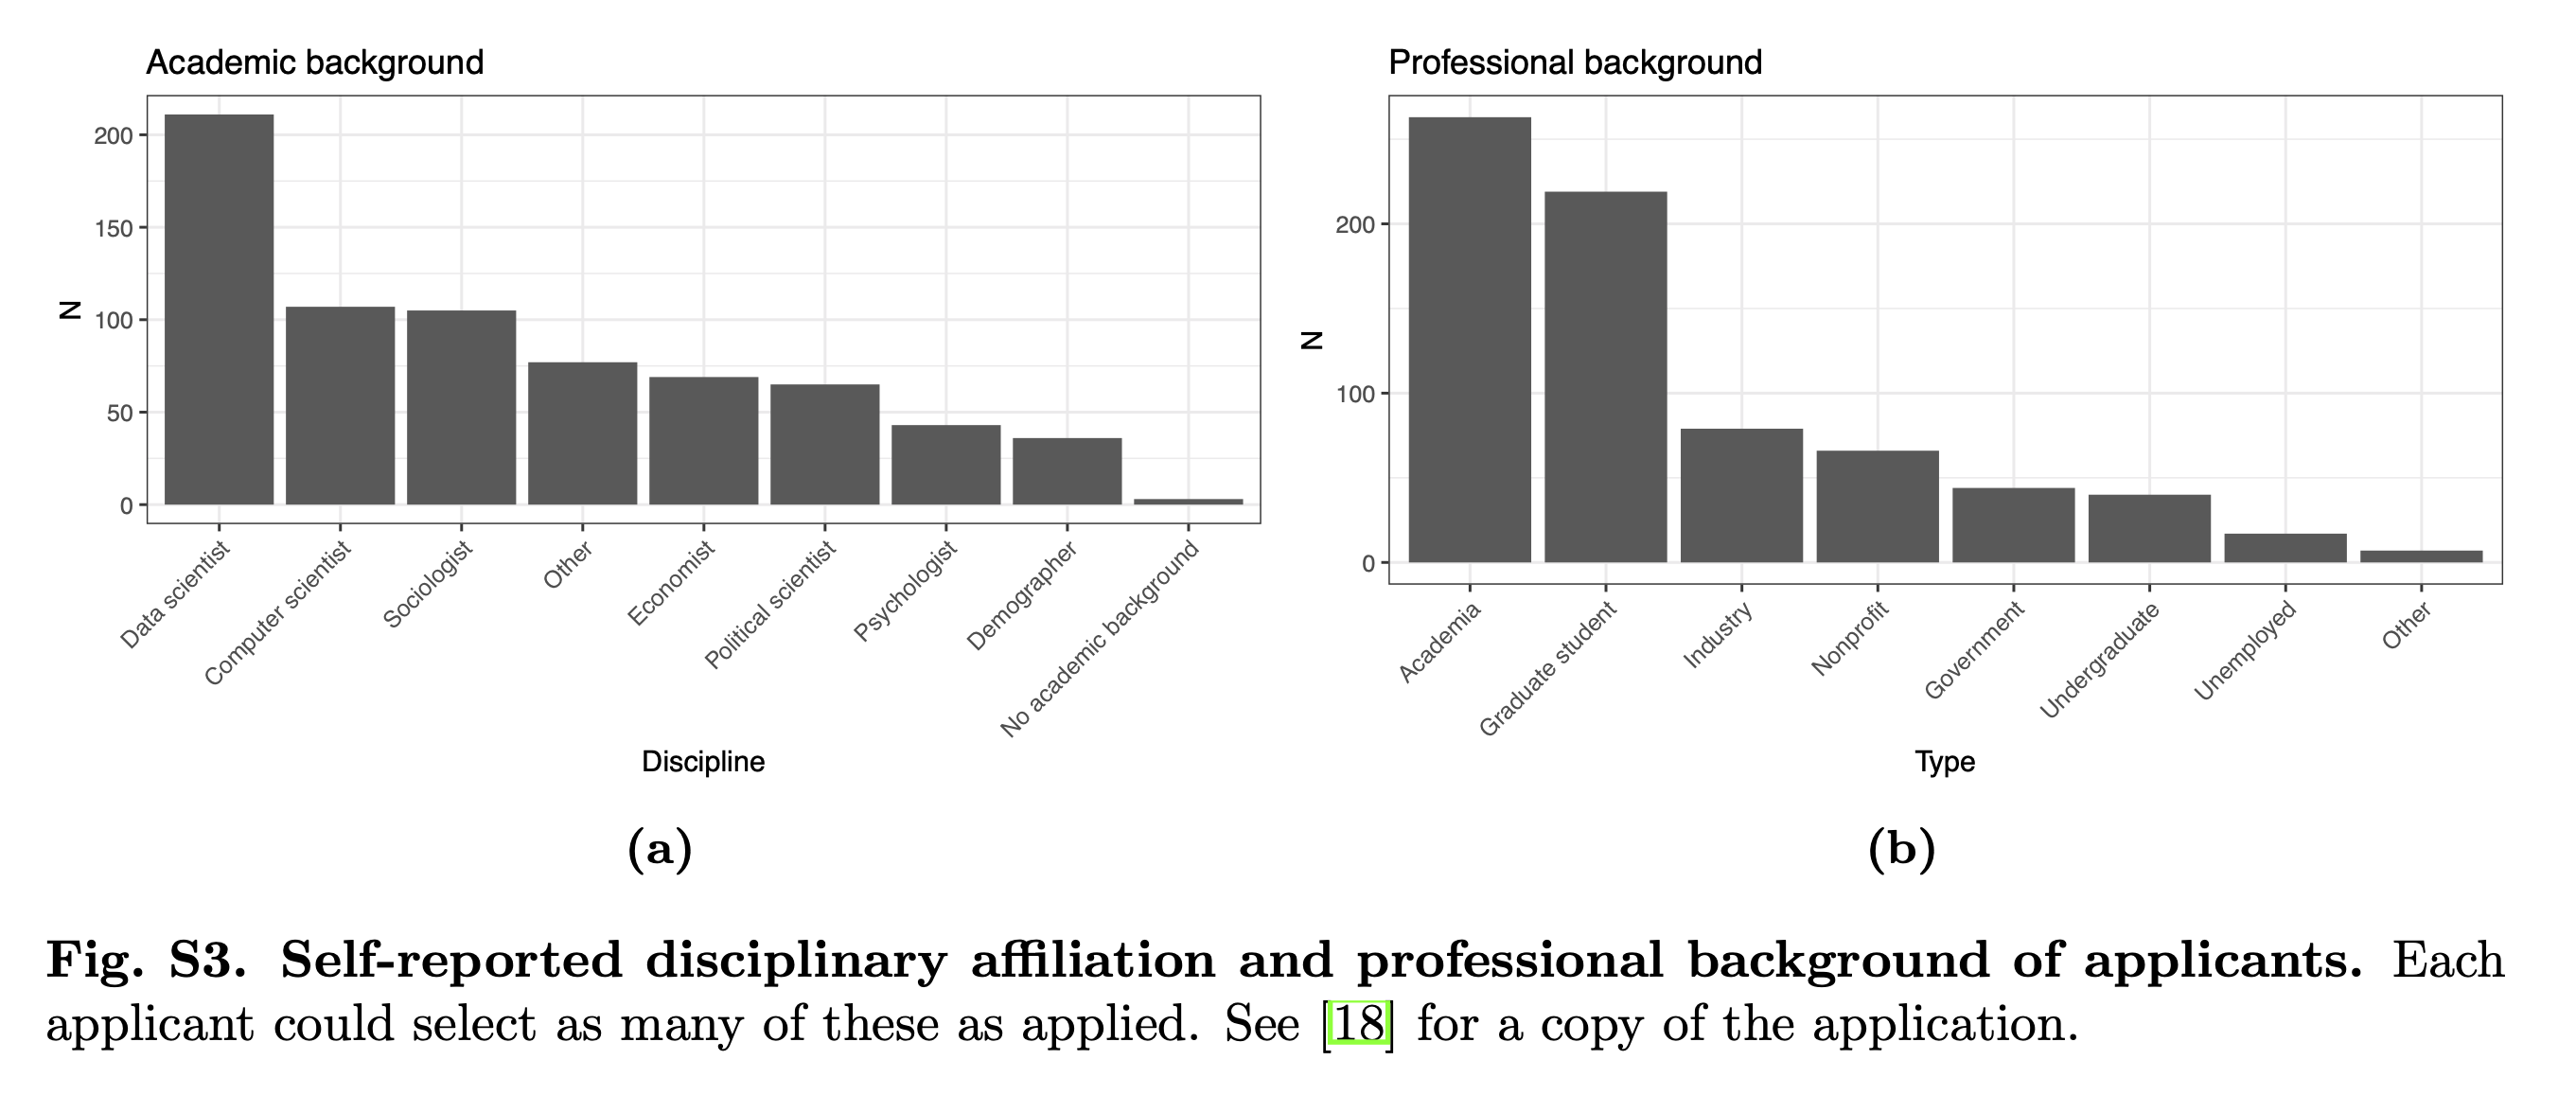
\includegraphics[width = \textwidth]{figures/si_disciplines}
\end{frame}

\begin{frame}{Appendix}
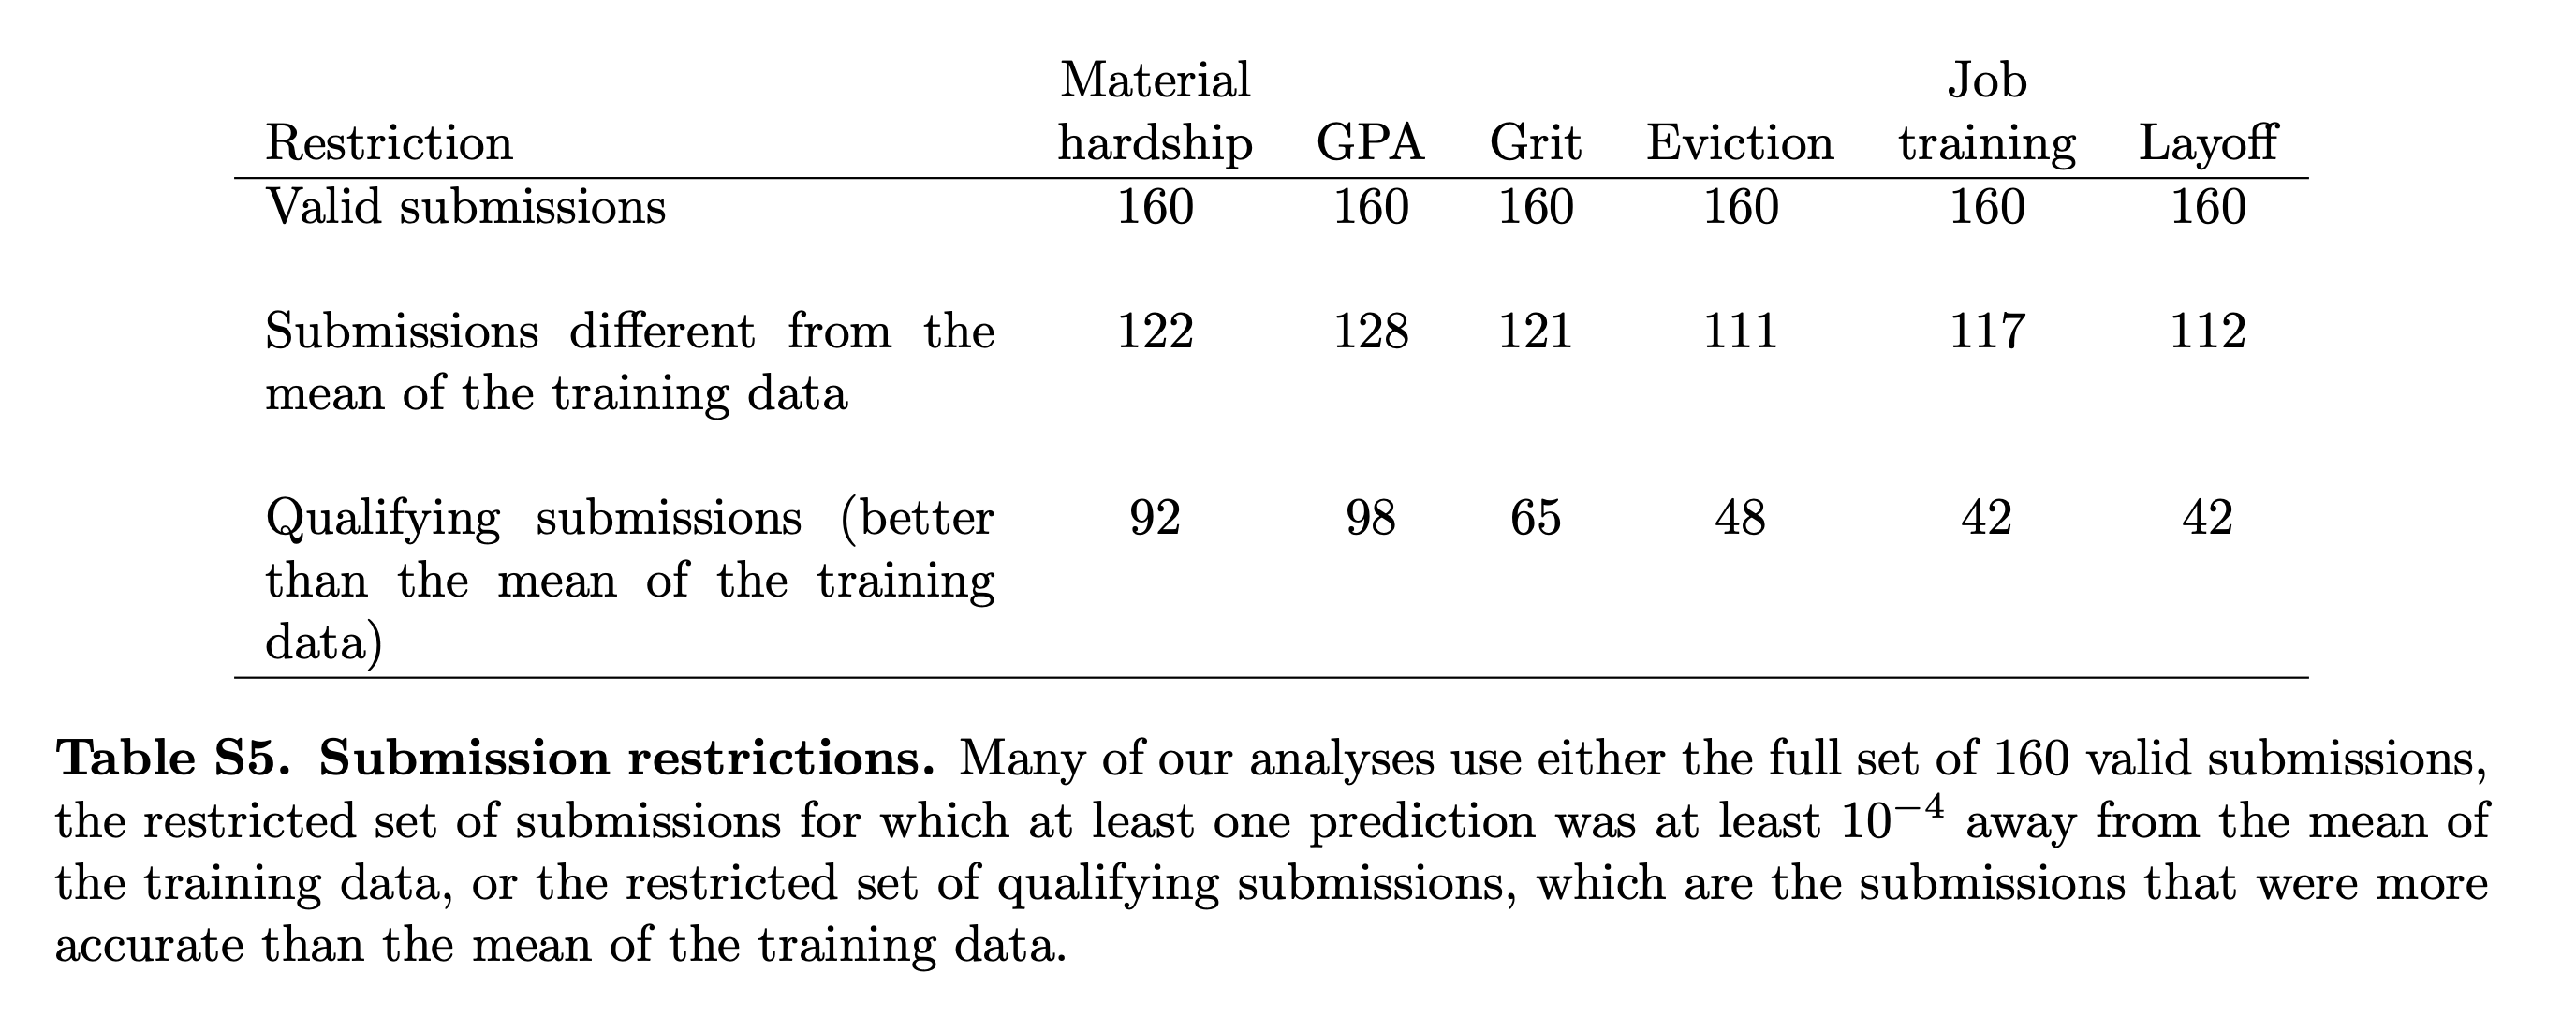
\includegraphics[width = \textwidth]{figures/si_qualifying_table}
\end{frame}

\begin{frame}{Appendix}
\centering
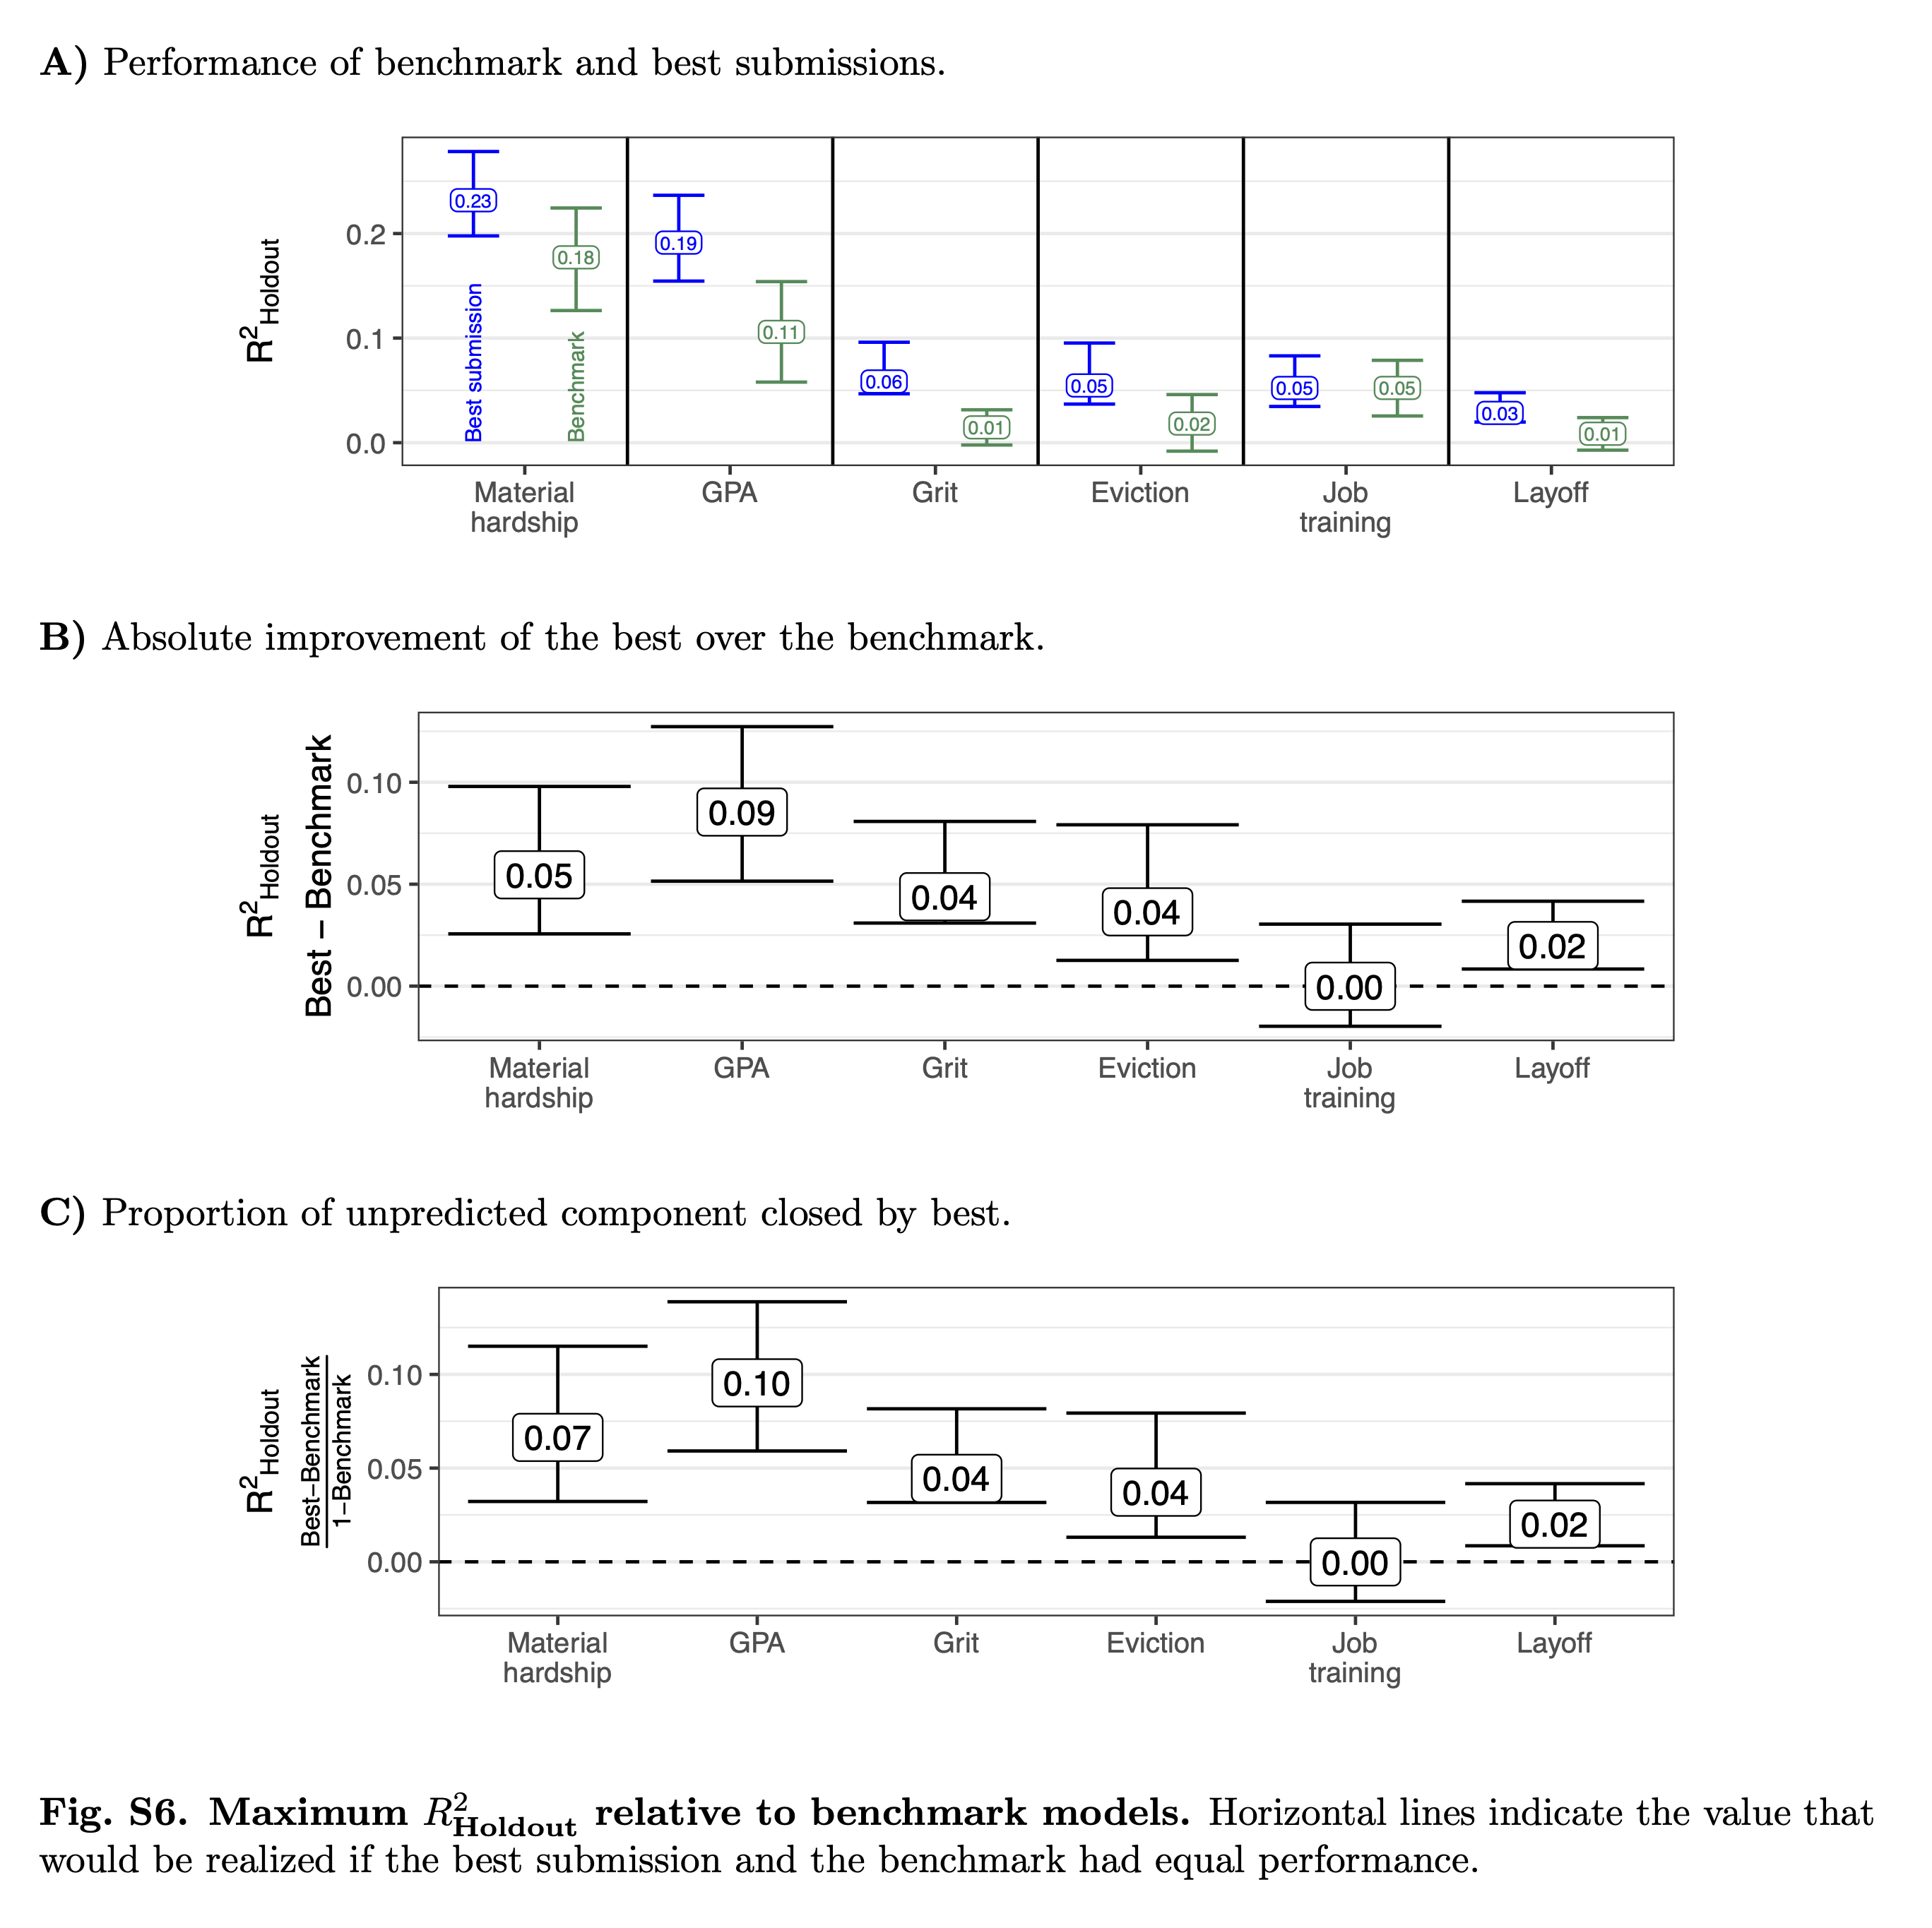
\includegraphics[height = .8\textheight]{figures/si_best_vs_benchmark}
\end{frame}

\begin{frame}{Appendix}
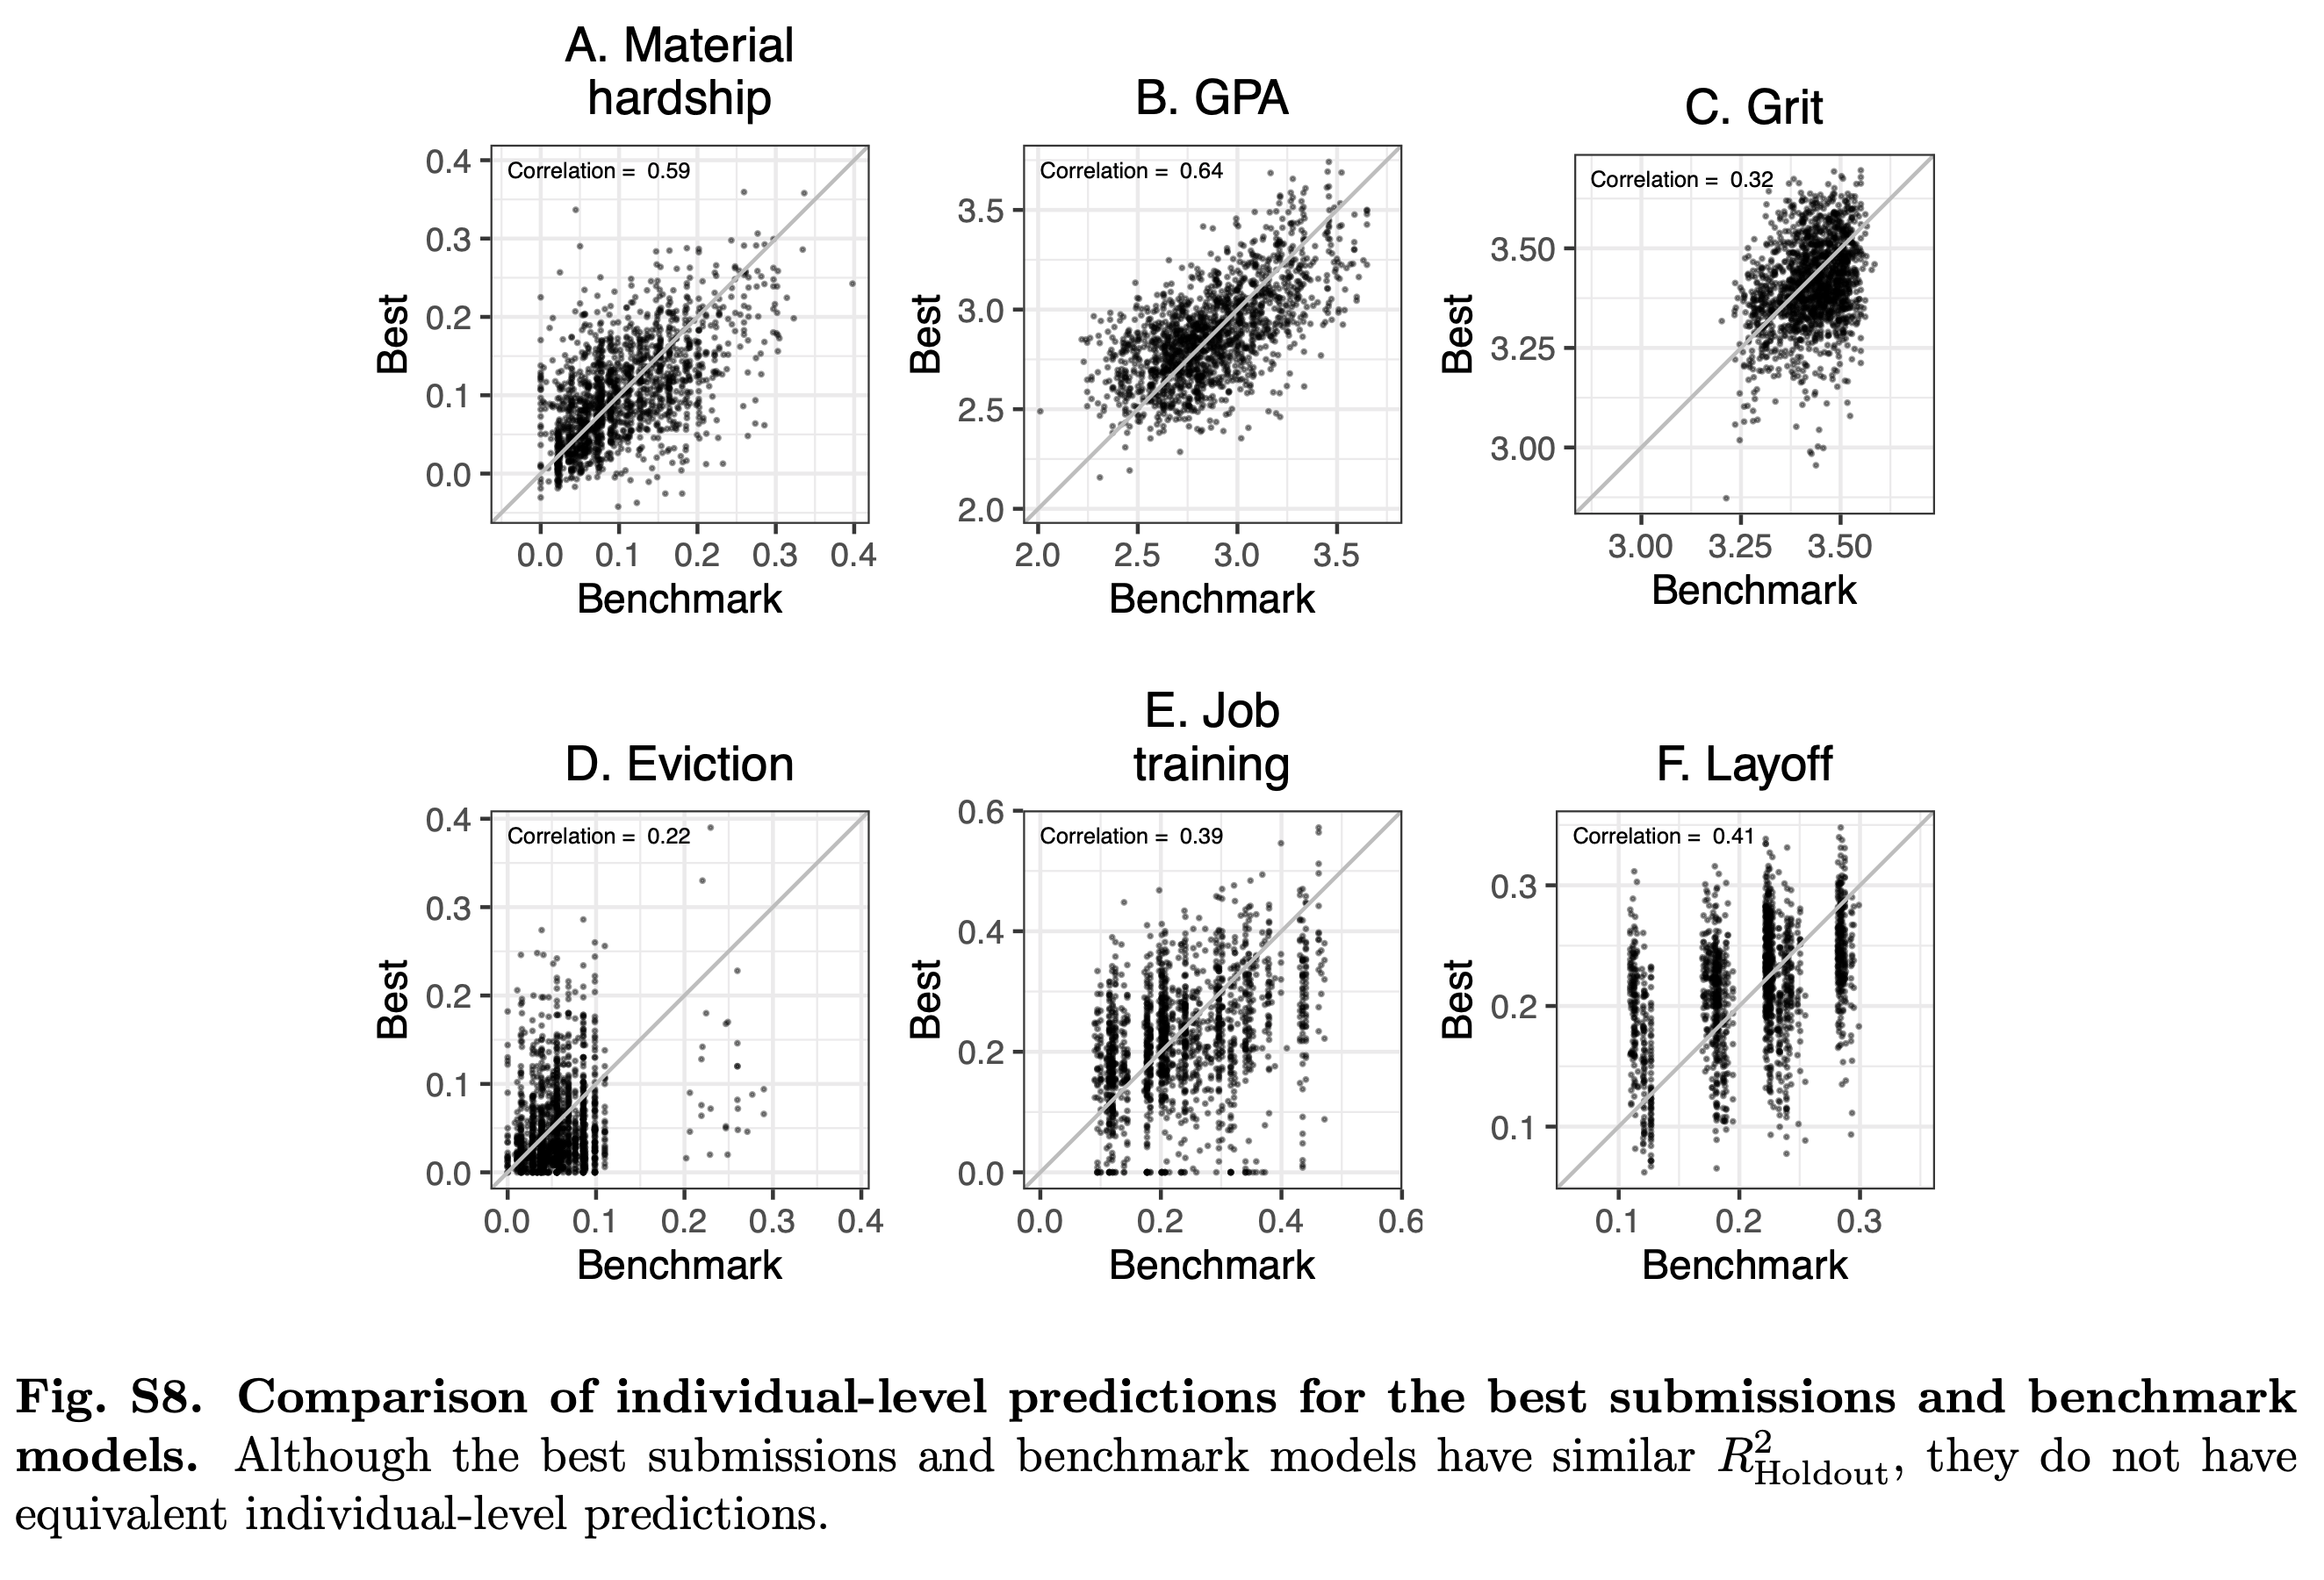
\includegraphics[width = \textwidth]{figures/si_best_benchmark_scatter}
\end{frame}

\begin{frame}{Appendix}
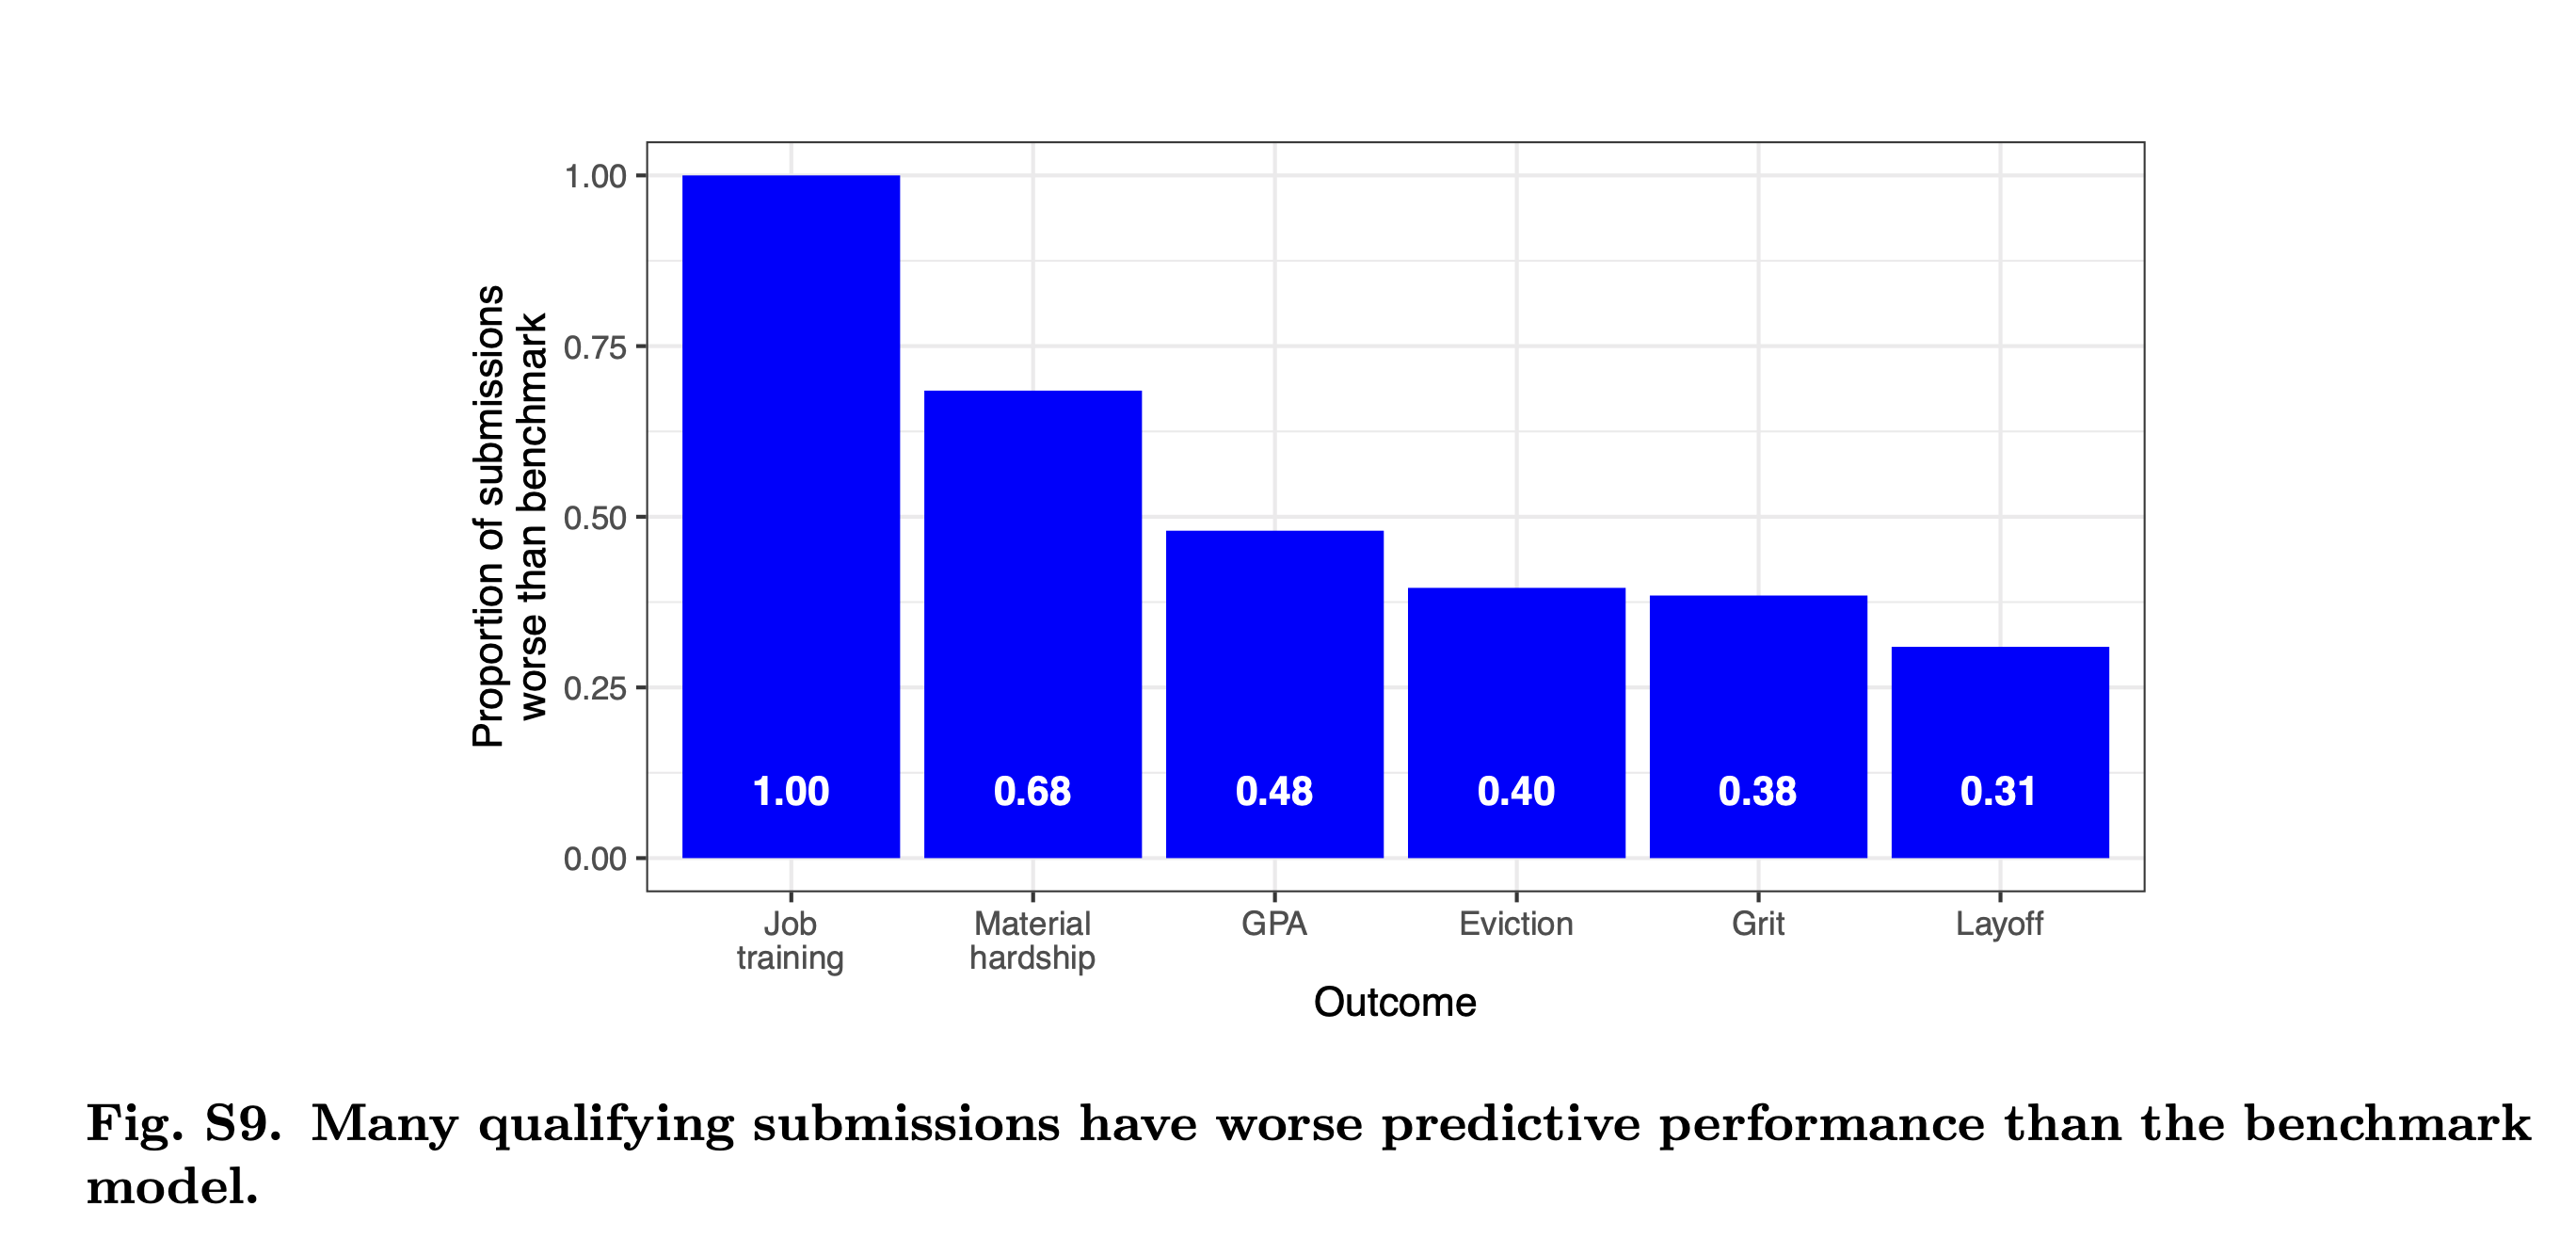
\includegraphics[width = \textwidth]{figures/si_worse_than_benchmark}
\end{frame}

\begin{frame}{Appendix}
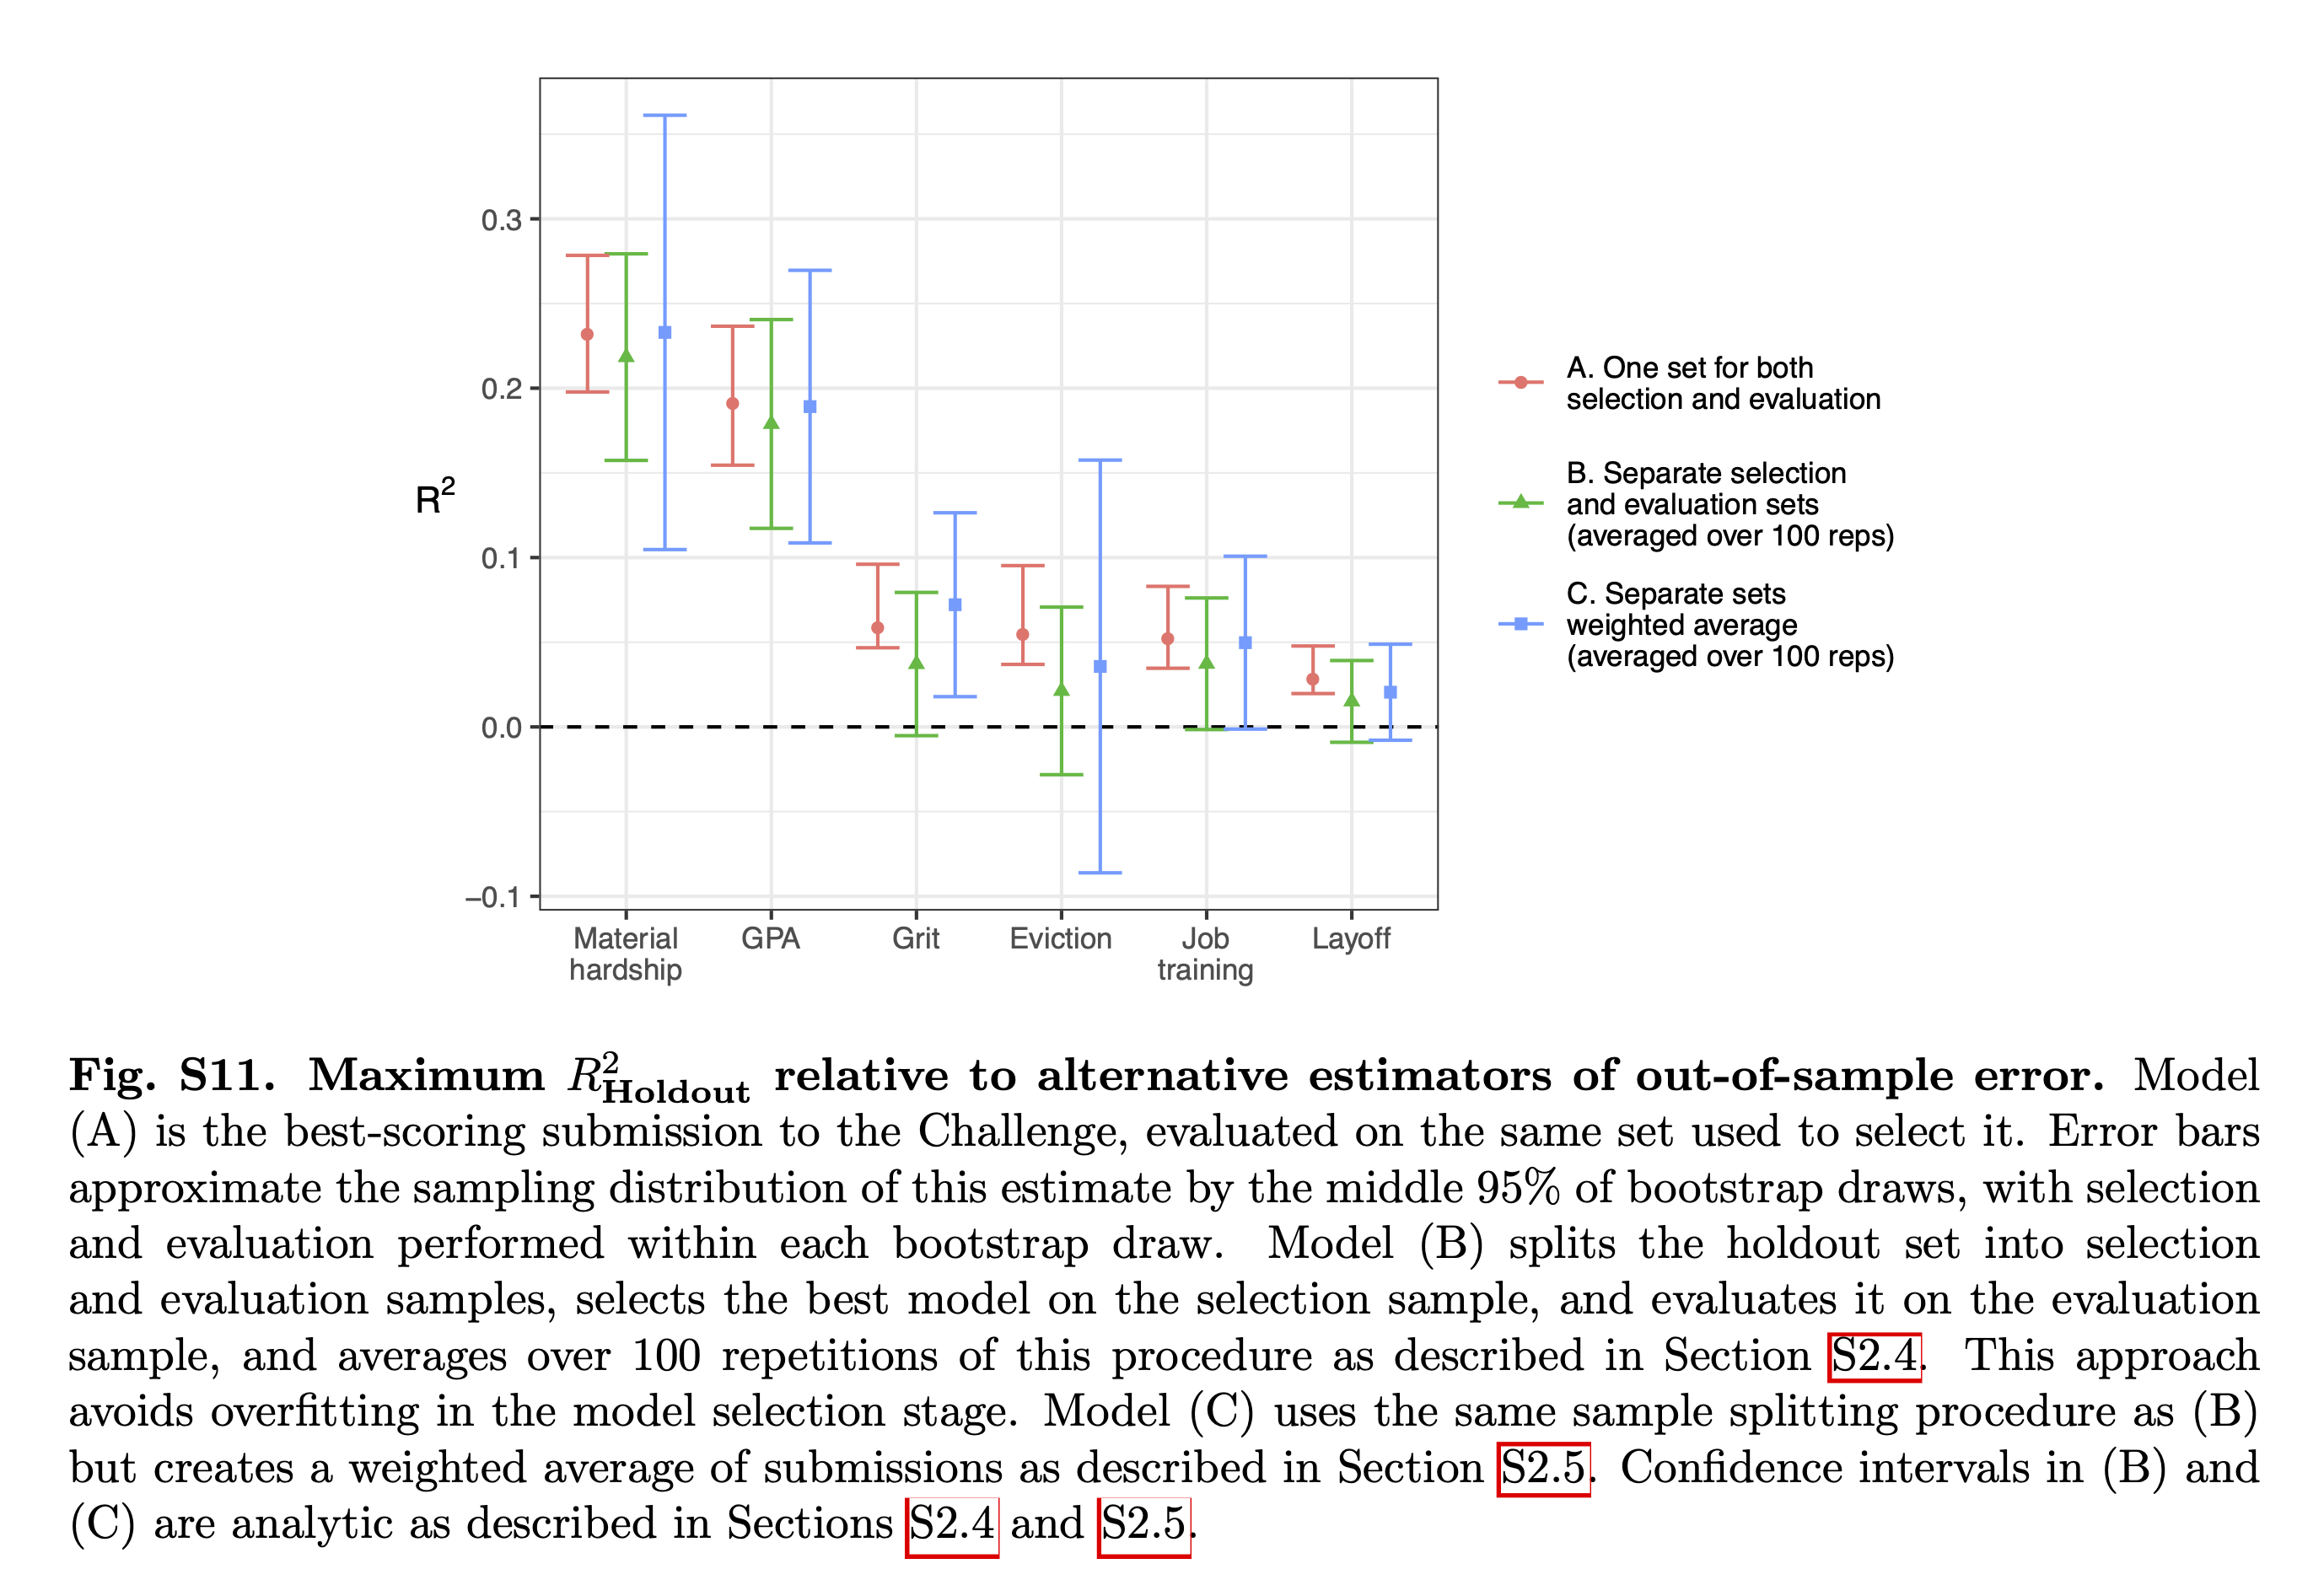
\includegraphics[width = \textwidth]{figures/si_ensemble}
\end{frame}

\begin{frame}{Appendix}
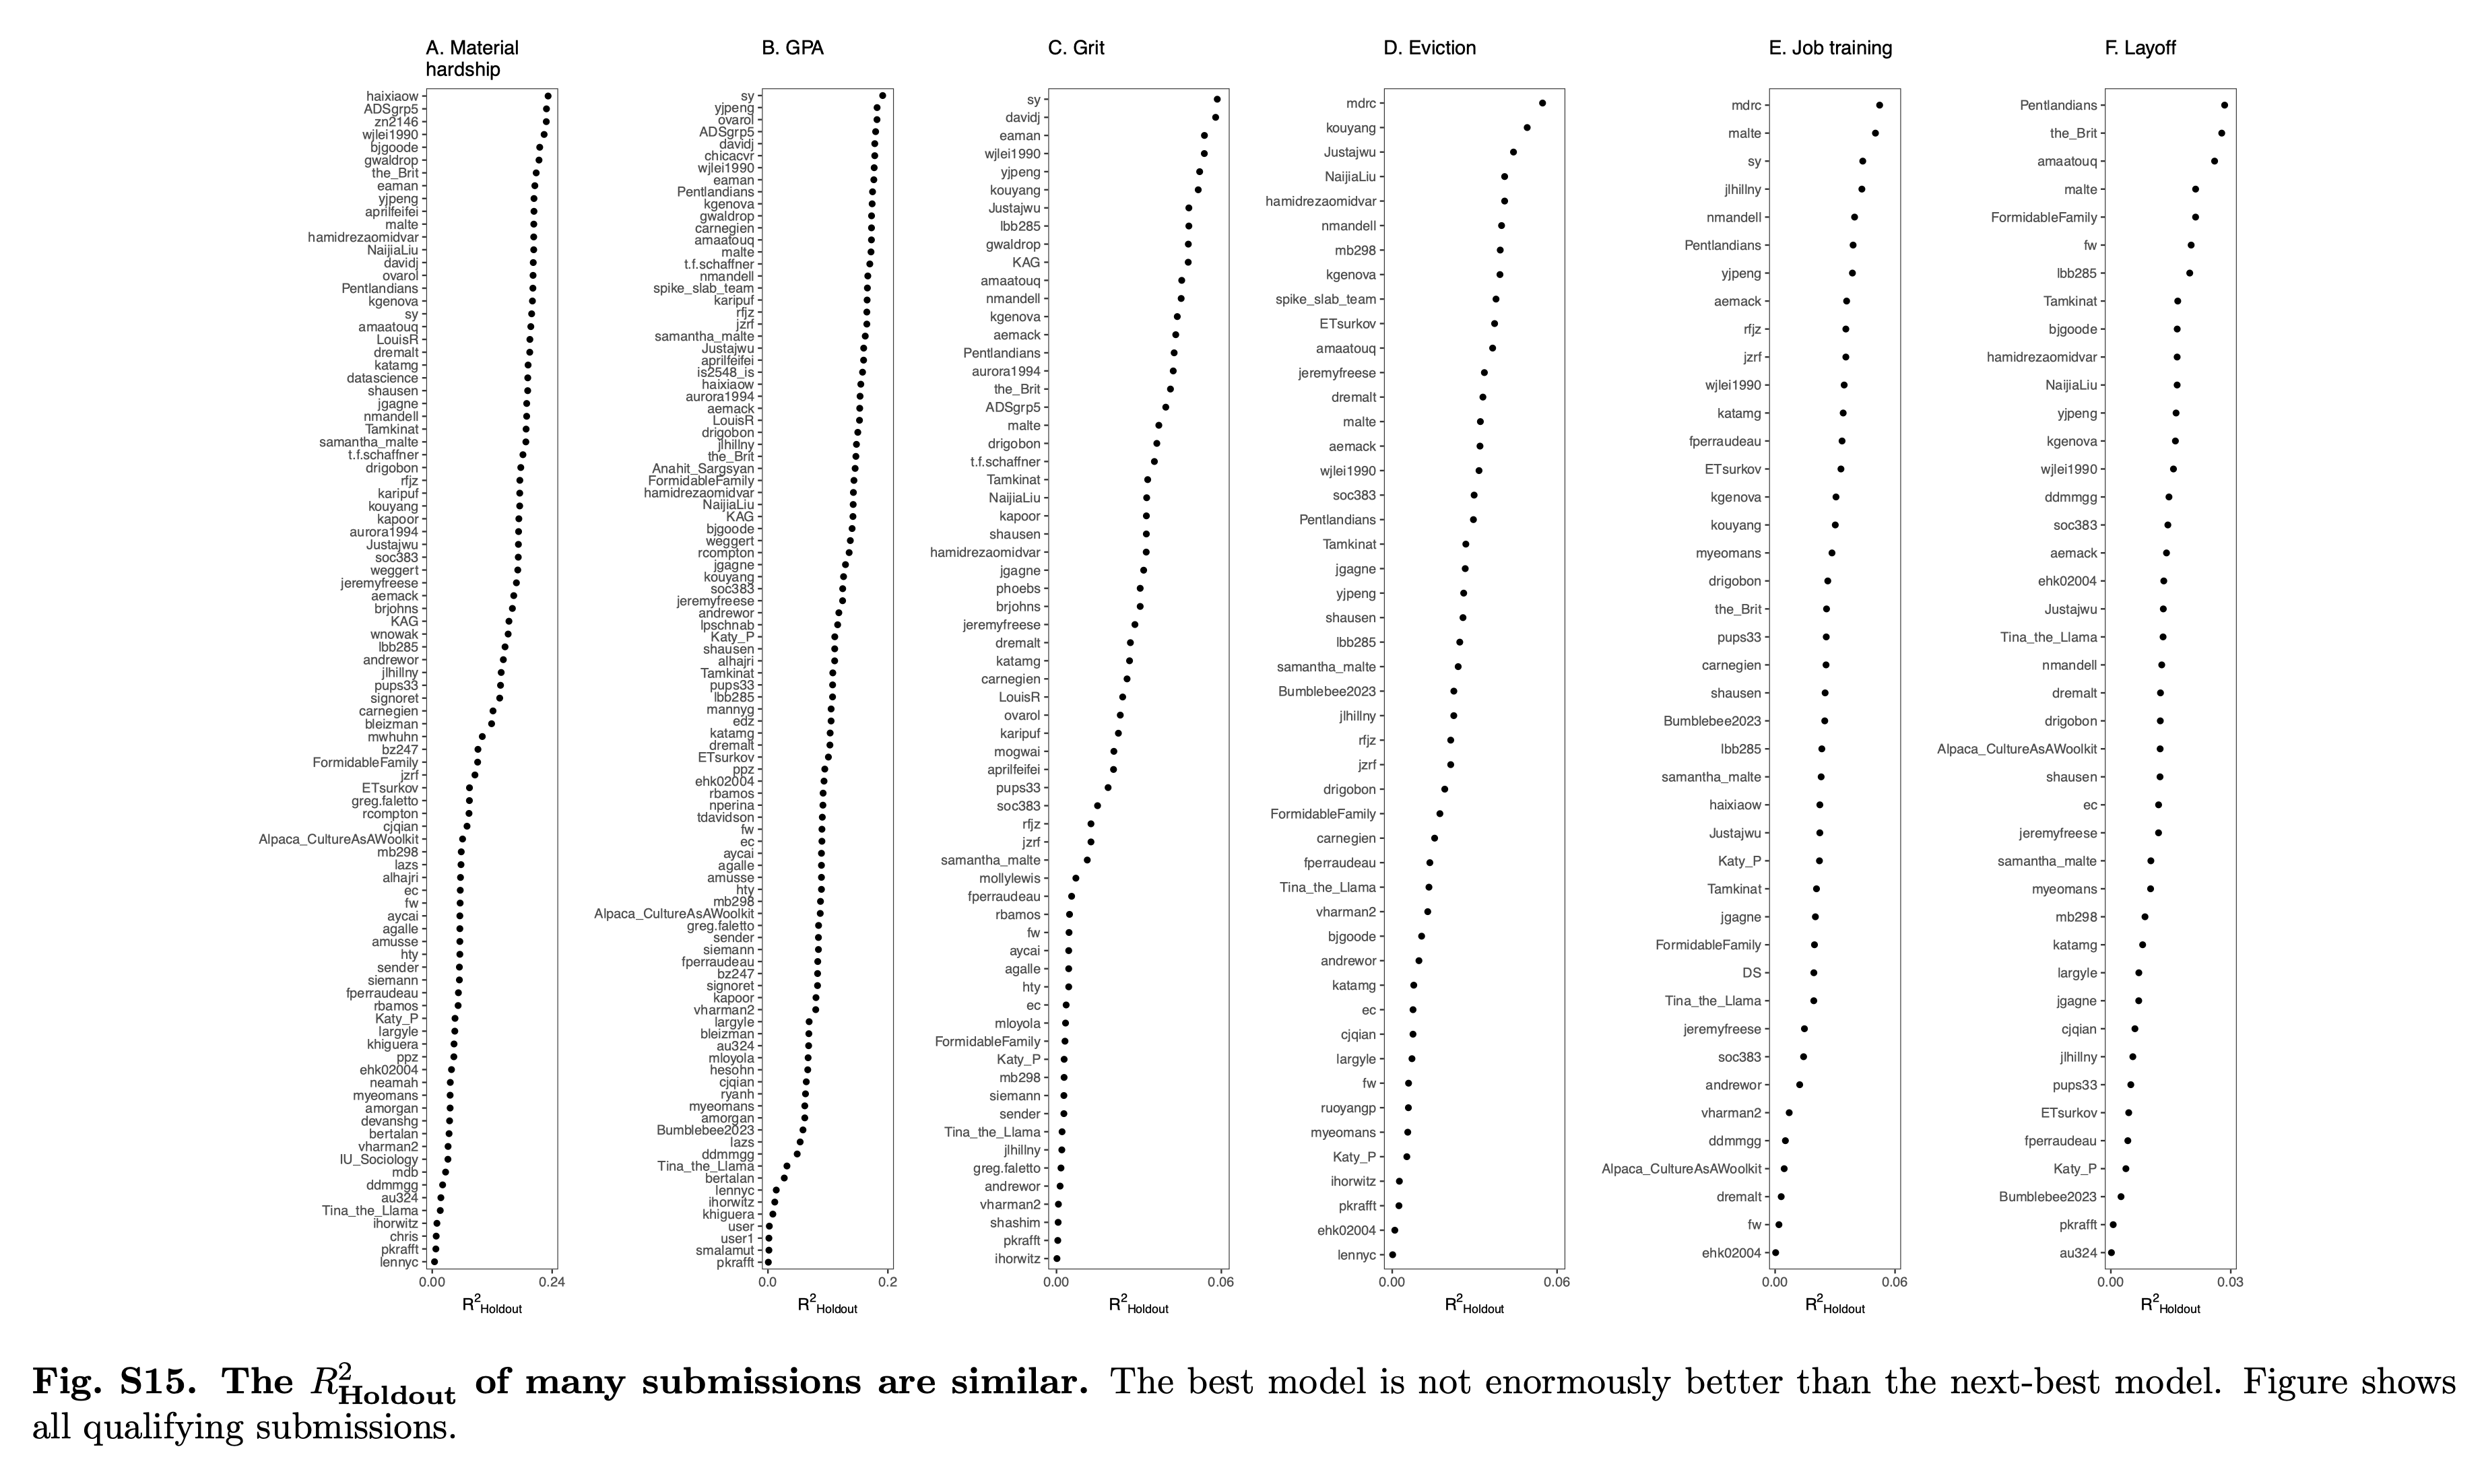
\includegraphics[width = \textwidth]{figures/si_best_teams}
\end{frame}

\begin{frame}{Appendix}
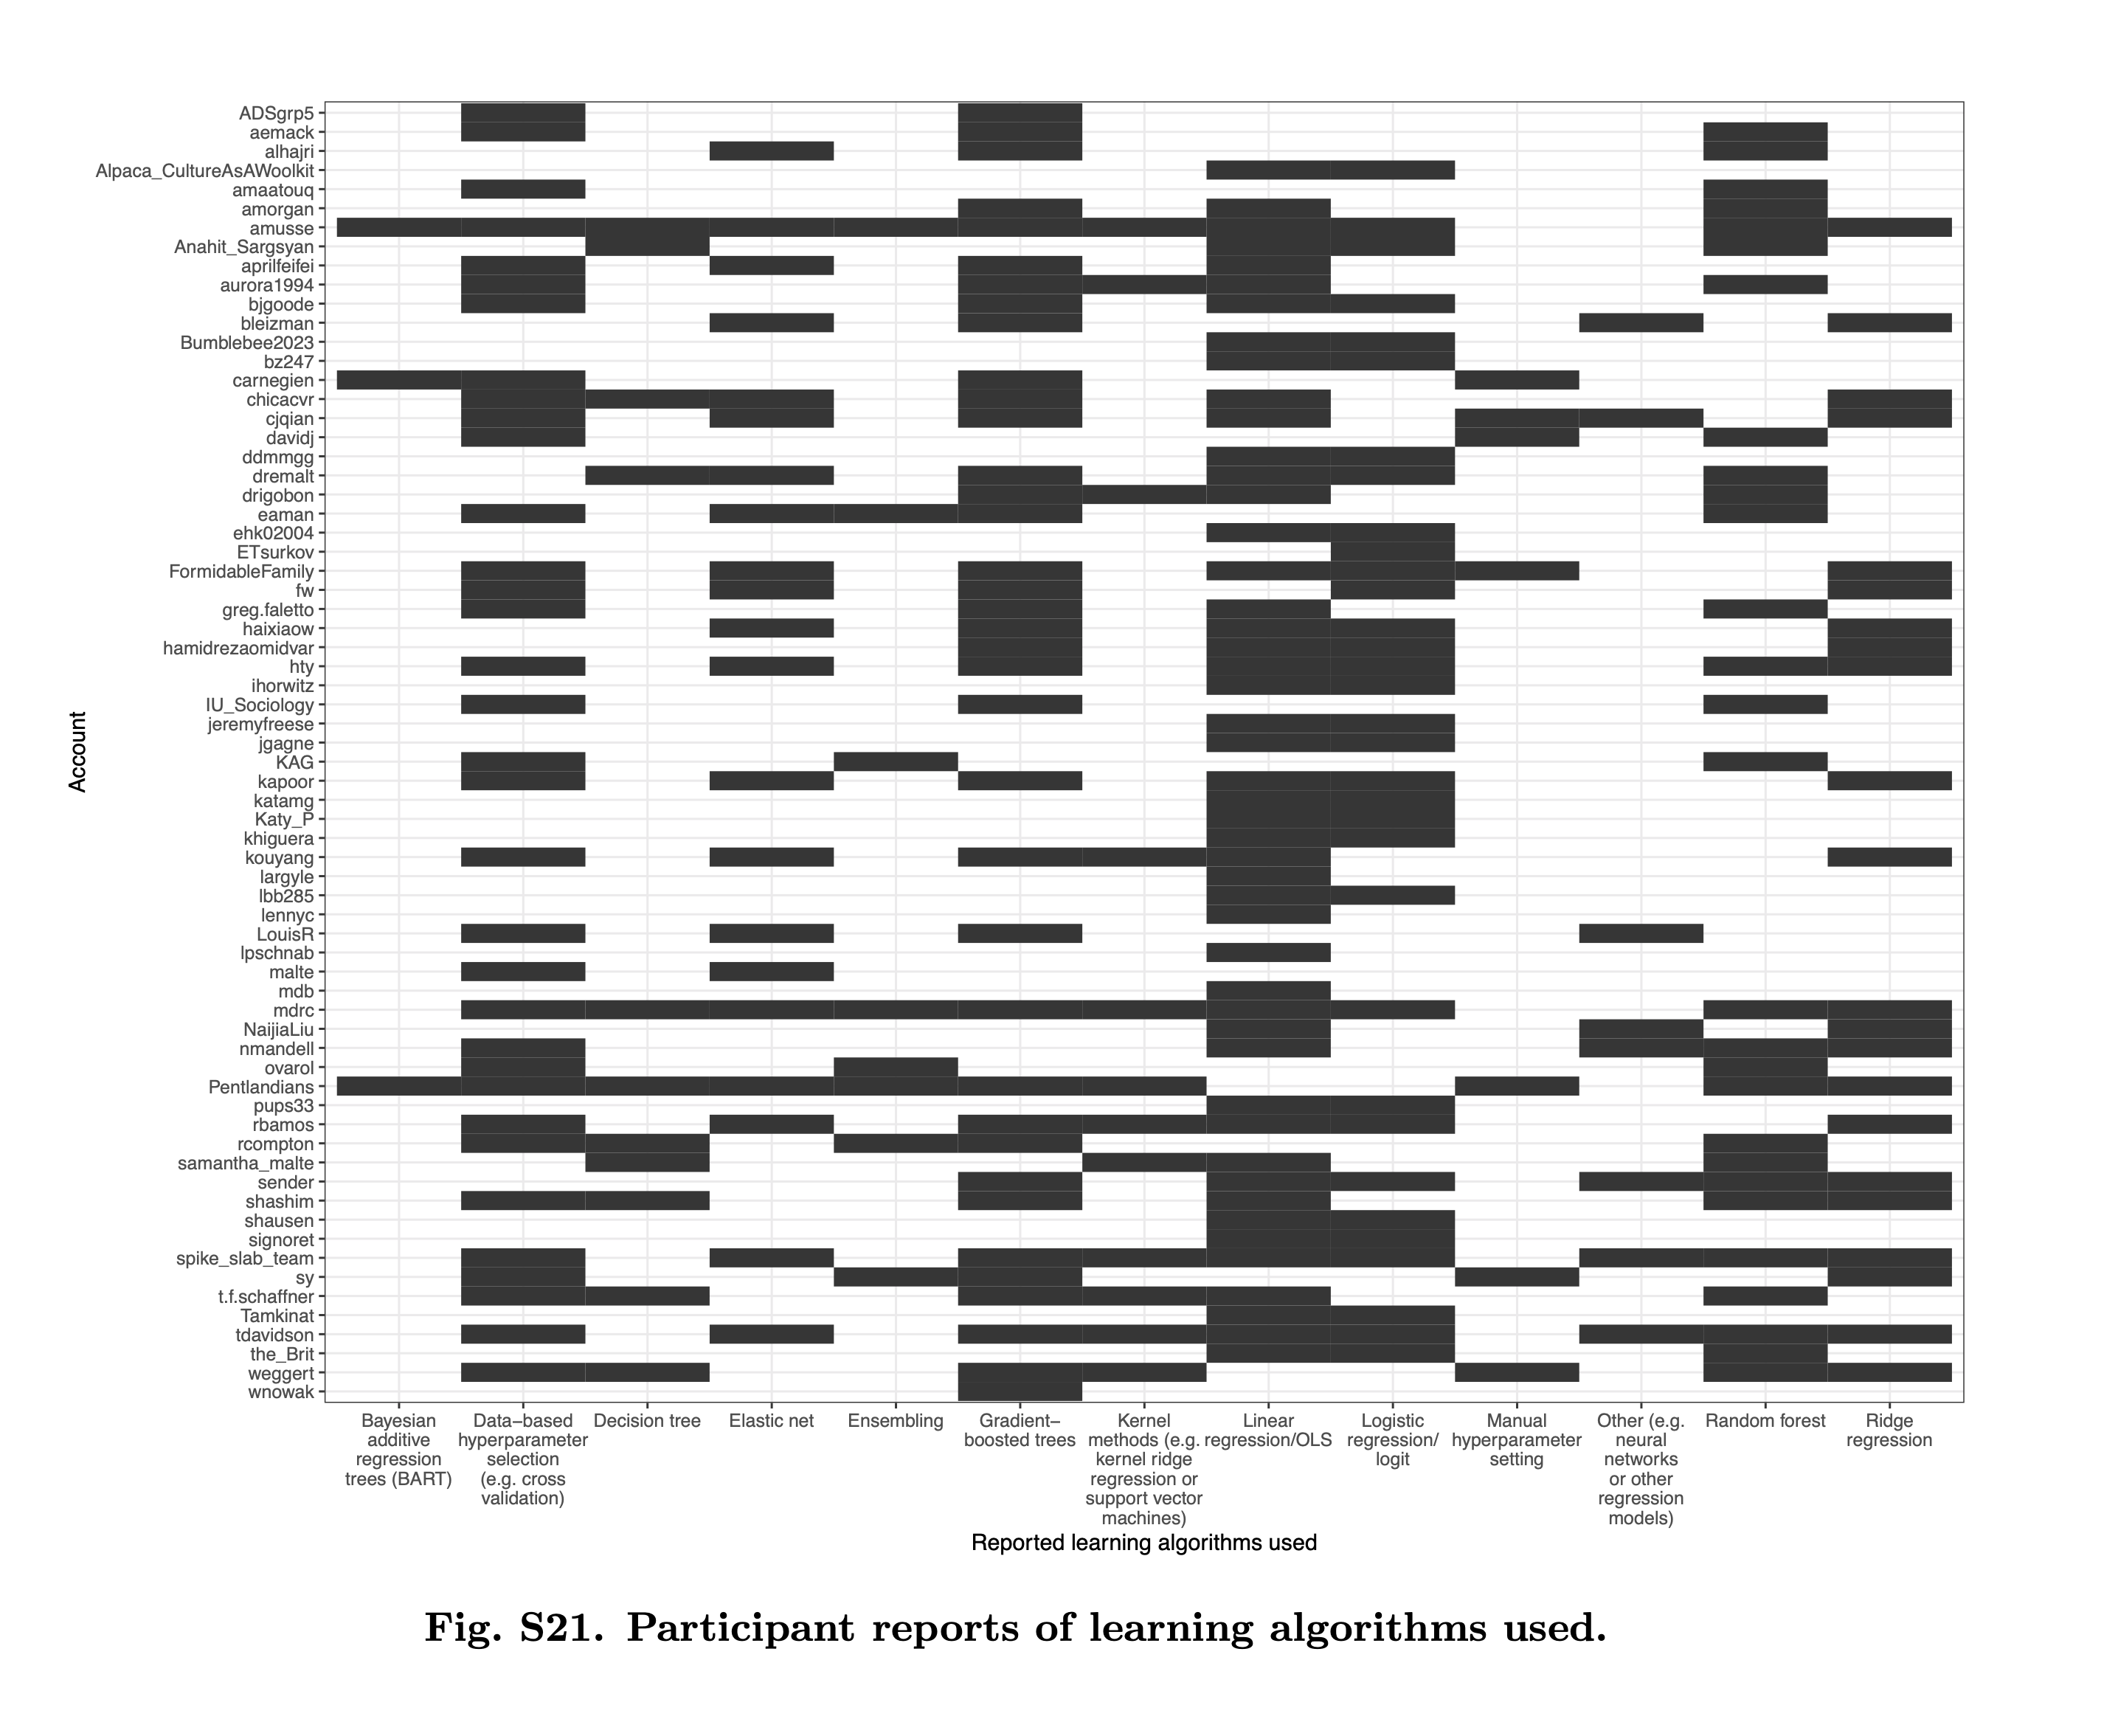
\includegraphics[width = \textwidth]{figures/si_algorithms}
\end{frame}


\end{document}

